\documentclass[preview]{standalone}
\usepackage{amssymb, amsthm}
\usepackage{mathtools}
\usepackage{bm}
\usepackage{standalone}


\begin{document}


\section{Theorems}


% ============================== 0062 Theorem 2320 ================================
\subsection[\texorpdfstring{$\gamma [\alpha]$ is strictly increasing...}
        {If a function is strictly increasing...}
    ]{
        \color{section}Theorem 62. \color{black} If \bm{$\gamma [\alpha]$} is strictly increasing...
    }
\documentclass[preview]{standalone}
\usepackage{amssymb, amsthm}
\usepackage{mathtools}
\usepackage{bm}


\newtheorem{theorem}{Theorem}
\renewcommand\qedsymbol{$\blacksquare$}


\begin{document}


\begin{theorem}[\textbf{2320}]
    Let \bm{$\gamma$} be a function \bm{$\gamma : \mathbb{R} \rightarrow \mathbb{R^+}$}.
    %such that
    % \begin{equation*}
    %     \forall \alpha
    %         \Big \langle \gamma [ \alpha ] > 0 \Big \rangle
    % \end{equation*}
    \\
    Let \bm{$\delta$} be the function \bm{$\delta: \mathbb{R} \rightarrow \mathbb{R}$} 
    defined by 
    \bm{$\delta [ \alpha ] = \frac{1}{\gamma[\alpha]}$}. 
    \begin{center}
        \bm{$\gamma[\alpha]$} is strictly increasing 
        if and only if 
        \bm{$\delta[\alpha]$} is strictly decreasing.
    \end{center}
\end{theorem}

\begin{proof}
    Suppose there exist real numbers \bm{$\alpha$} and \bm{$\beta$} such that 
    \bm{$\alpha < \beta$}, 
    and suppose that \bm{$\gamma[\alpha] < \gamma[\beta]$}. 
    \bm{$\gamma$} is a strictly increasing real-valued function by definition.
    By the multiplicative compatibility law from the order axioms, 
    %multiplying both sides of the latter inequality by 
    %\bm{$\frac{1}{\gamma[\alpha]\cdot\gamma[\beta]}$}
    \begin{equation*}
        \Bigg\{
            \left(
                \frac{\gamma[\alpha]}{\gamma[\alpha] \cdot \gamma[\beta]} 
            \right)
                    < 
            \left(
                \frac{\gamma[\beta]}{\gamma[\alpha] \cdot \gamma[\beta]}
            \right)
        \Bigg\}
            \equiv
        \Bigg\{
            \left(
                \frac{1}{\gamma[\beta]}
            \right)
                <
            \left(
                \frac{1}{\gamma[\alpha]}
            \right)
        \Bigg\}
            \equiv
    \end{equation*}
    \begin{equation*}
        \Bigg\{
            \bigg( \delta[\beta] \bigg)
                < 
            \bigg( \delta[\alpha] \bigg)
        \Bigg\}
    \end{equation*}
    Thus, \bm{$\delta$} is a strictly decreasing real-valued function,
    by definition. The converse can be proven by multiplying that inequality
    \bm{$\delta[\alpha] > \delta[\beta]$} by \bm{$\gamma[\alpha]\gamma[\beta]$},
    by the multiplicative compatibility law from the order axioms,
    \begin{equation*}
        \Bigg\{
            \left(
                \frac{1 \cdot \gamma[\alpha] \cdot \gamma[\beta]}{\gamma[\alpha]}
            \right)
                >
            \left(
                \frac{1 \cdot \gamma[\alpha] \cdot \gamma[\beta]}{\gamma[\beta]}
            \right)
        \Bigg\}
            \equiv
        \Bigg\{
            \bigg( \gamma[\beta] \bigg) 
                > 
            \bigg( \gamma[\alpha] \bigg)
        \Bigg\}
    \end{equation*}
    Thus, \bm{$\gamma$} is a strictly increasing real-valued function, by definition
    \bm{$\therefore \text{\space} \gamma[\alpha]$} is strictly increasing 
    if and only if 
    \bm{$\delta[\alpha]$} is strictly decreasing.
\end{proof}

    
\end{document}
\pagebreak


% ============================== 0063 Theorem 2321 ================================
\subsection[\texorpdfstring{$\gamma [\alpha]$ is strictly decreasing...}
        {If a function is strictly decreasing...}
    ]{
        \color{section}Theorem 63. \color{black} If \bm{$\gamma [\alpha]$} is strictly decreasing...
    }
\documentclass[preview]{standalone}
\usepackage{amssymb, amsthm}
\usepackage{mathtools}
\usepackage{bm}


\newtheorem{theorem}{Theorem}
\renewcommand\qedsymbol{$\blacksquare$}


\begin{document}


\begin{theorem}[\textbf{2321}]
    Let \bm{$\gamma$} be the function \bm{$\gamma : \mathbb{R} \rightarrow \mathbb{R^+}$}.
    %, such that 
    % \begin{equation*}
    %     \forall \alpha \Big \langle
    %         \gamma[ \alpha ] > 0 \Big \rangle    
    % \end{equation*} 
    \\
    Let \bm{$\delta$} be the function \bm{$\delta : \mathbb{R} \rightarrow \mathbb{R}$} 
    defined by \bm{$\delta[\alpha] = \frac{1}{\gamma[\alpha]}$}. 
    \begin{center}
        \bm{$\gamma[\alpha]$} is strictly decreasing 
            if and only if 
        \bm{$\delta[\alpha]$} is strictly increasing.
    \end{center}
\end{theorem}

\begin{proof}
    Suppose there exist real numbers \bm{$\alpha$} and \bm{$\beta$} such that 
    \bm{$\alpha < \beta$}, and suppose that 
    \bm{$\gamma[ \alpha ] > \gamma[ \beta ]$}. \bm{$\gamma$} is a strictly decreasing real-valued function by definition. 
    By the multiplicative compatibility law from the order axioms, 
    Multiplying both sides of the latter inequality by \bm{$\frac{1}{\gamma[\alpha] \cdot \gamma[\beta]}$}
    \begin{equation*}
        \Bigg\{
            \left(
                \frac{\gamma[\alpha]}{\gamma[\alpha] \cdot \gamma[\beta]}
            \right)
                >
            \left(
                \frac{\gamma[\beta]}{\gamma[\alpha] \cdot \gamma[\beta]}
            \right)  
        \Bigg\}
            \equiv
        \Bigg\{
            \left(
                \frac{1}{\gamma[\beta]}
            \right)
                >
            \left(
                \frac{1}{\gamma[\alpha]}
            \right)
        \Bigg\}
            \equiv
    \end{equation*}
    \begin{equation*}
        \Bigg\{
            \bigg(
                \delta[\beta]
            \bigg)
                >
            \bigg(
                \delta[\alpha]
            \bigg)
        \Bigg\}
    \end{equation*}
    Thus, \bm{$\delta$} is a strictly increasing real-valued function,
    by defintion.
    The converse can be proven by multiplying that inequality
    \bm{$\delta[\alpha] < \delta[\beta]$} by \bm{$\gamma[\alpha]\gamma[\beta]$},
    by the multiplicative compatibility law from the order axioms,
    \begin{equation*}
        \Bigg\{
            \bigg(
                \frac{1 \cdot \gamma[\alpha] \cdot \gamma[\beta]}{\gamma[\alpha]}
                    <
                \frac{1 \cdot \gamma[\alpha] \cdot \gamma[\beta]}{\gamma[\beta]}
            \bigg)
        \Bigg\}
            \equiv
        \Bigg\{
            \bigg(
                \gamma[\beta]
            \bigg)
                <
            \bigg(
                \gamma[\alpha]
            \bigg)
        \Bigg\} 
    \end{equation*}
    Thus, \bm{$\gamma$} is a strictly decreasing real-valued function, by defintion
    \bm{$\therefore \text{\space} \gamma[\alpha]$} is strictly decreasing
    if and only if
    \bm{$\delta[\alpha]$} is strictly increasing.
\end{proof}


\end{document}
\sep


% ============================== 0064 Theorem 2324 ================================
\subsection[Exponentiation is not invertible.]
    {
        \color{section}Theorem 64. \color{black} Exponentiation is not invertible.
    }
\documentclass[preview]{standalone}
\usepackage{amssymb, amsthm}
\usepackage{mathtools}
\usepackage{bm}


\newtheorem{theorem}{Theorem}
\renewcommand\qedsymbol{$\blacksquare$}


\begin{document}


\begin{theorem}[\textbf{2324}]
    Let \bm{$\alpha$} be the function 
    \bm{$\alpha: \mathbb{R} \rightarrow \mathbb{R}$}
    defined by \bm{$\alpha[\lambda] = \epsilon ^\lambda$}. 
    \begin{center}
        \bm{$\alpha[\lambda]$} is not invertible.
    \end{center}
\end{theorem}

\begin{proof}
    \begin{equation*}
        \Big \langle \alpha[\lambda] = \epsilon ^\lambda \Big \rangle
            \rightarrow
        \bigg[
            \Big \langle \alpha ^{-1}[\lambda] \Big \rangle 
                =
            \Big \langle \log_{\epsilon} \lambda \Big \rangle
        \bigg]
    \end{equation*}
    The domain for \bm{$\alpha ^{-1}[\lambda]$} is \bm{$\mathbb{R}$}, by definition. 
    But logarithmic functions are undefined for negative-valued domains.
    Thus, \bm{$\alpha[\lambda]$} cannot be bijective, 
    so \bm{$\alpha[\lambda]$} is not invertible.
\end{proof}


\end{document}
\pagebreak


% ============================== 0065 Theorem 2325 ================================
\subsection[Absolute value is not invertible.]
    {
        \color{section}Theorem 65. \color{black} Absolute value is not invertible.
    }
\documentclass[preview]{standalone}
\usepackage{amssymb, amsthm}
\usepackage{mathtools}
\usepackage{bm}


\newtheorem{theorem}{Theorem}
\renewcommand\qedsymbol{$\blacksquare$}


\begin{document}


\begin{theorem}[\textbf{2325}]
    Let \bm{$\alpha$} be a function 
    \bm{$\alpha : \mathbb{R} \rightarrow \mathbb{R}$}
    defined by \bm{$\alpha[\lambda] = |\lambda|$}. 
    \begin{center}
        \bm{$\alpha[\lambda]$} is not invertible.
    \end{center}
\end{theorem}

\begin{proof}
    Let \bm{$\lambda$} be a postive real number. 
    By the definition for \bm{$\alpha$}, 
    \begin{equation*}
        \Big \langle \alpha[\lambda] = \lambda \Big \rangle
            \land
        \Big \langle \alpha[-1 \cdot \lambda] = \lambda \Big \rangle
    \end{equation*}
    So if \bm{$\alpha$} had an inverse, then
    \begin{equation*}
        \Big \langle \alpha ^{-1}[\lambda] = \lambda \Big \rangle
            \lor 
        \Big \langle \alpha ^{-1}[\lambda] = -1 \cdot \lambda \Big \rangle
    \end{equation*}
    Thus, \bm{$\alpha ^{-1}$} is not a function by definition.
\end{proof}


\end{document}
\sep


% ============================== 0066 Theorem 2329a ================================
\subsection[The composition of injective functions is injective.]
    {
        \color{section}Theorem 66. \color{black} The composition of injective functions.
    }
\documentclass[preview]{standalone}
\usepackage{amssymb, amsthm}
\usepackage{mathtools}
\usepackage{bm}


\newtheorem{theorem}{Theorem}
\renewcommand\qedsymbol{$\blacksquare$}


\begin{document}


\begin{theorem}[\textbf{2329a}]
    Let \bm{$\lambda$} be a function 
    \bm{$\lambda: \Delta \rightarrow \mathrm{A}$}, 
    and let \bm{$\epsilon$} be a function 
    \bm{$\epsilon: \Lambda \rightarrow \Delta$}. 
    \begin{center}
        If both \bm{$\lambda$} and \bm{$\epsilon$} are injective, 
        then \bm{$\big \langle \lambda \circ \epsilon \big \rangle$} is injective.
    \end{center}
\end{theorem}

\begin{proof}
    By the contrapositive.
    Suppose it were not the case that 
    \bm{$\big \langle \lambda \circ \epsilon \big \rangle$}
    were injective. 
    By the definition for injective functions, 
    with domain of discourse 
    \bm{$\big \langle \iota, \zeta \in \Lambda \big \rangle$}, that is
    \begin{equation*}
        \lnot \forall \iota \forall \zeta \bigg \langle 
            \Big[
                \big \langle \lambda \circ \epsilon \big \rangle [\iota] 
                    = 
                \big \langle \lambda \circ \epsilon \big \rangle [\zeta] 
            \Big]
                \rightarrow 
            \big \langle \iota = \zeta \big \rangle 
        \bigg \rangle
    \end{equation*}
    The composition of functions 
    \bm{$\big \langle \lambda \circ \epsilon \big \rangle [\iota]$} 
    is defined as \bm{$\lambda \big[ \epsilon (\iota) \big]$}. 
    Thus, we have the equivalent universal quantification
    \begin{equation*}
        \lnot \forall \iota \forall \zeta \bigg \langle 
            \Big[
                \lambda \big[ \epsilon (\iota) \big] 
                    = 
                \lambda \big[ \epsilon (\zeta) \big] 
            \Big]
                \rightarrow
            \big \langle \iota = \zeta \big \rangle
        \bigg \rangle
    \end{equation*}
    In other words, it follows from the negation of the direct consequent that 
    it is not the case that \bm{$\lambda$} is injective, 
    by the definition for injective functions. 
    This is sufficient to prove the logical negation of the direct hypothesis. 
    Thus, if both \bm{$\lambda$} and \bm{$\epsilon$} are injective, 
    then 
    \bm{$\big \langle \lambda \circ \epsilon \big \rangle$} 
    is injective.
\end{proof}


\end{document}
\pagebreak


% ============================== 0067 Theorem 2329b ================================
\begin{figure}[!h]
    \centering
    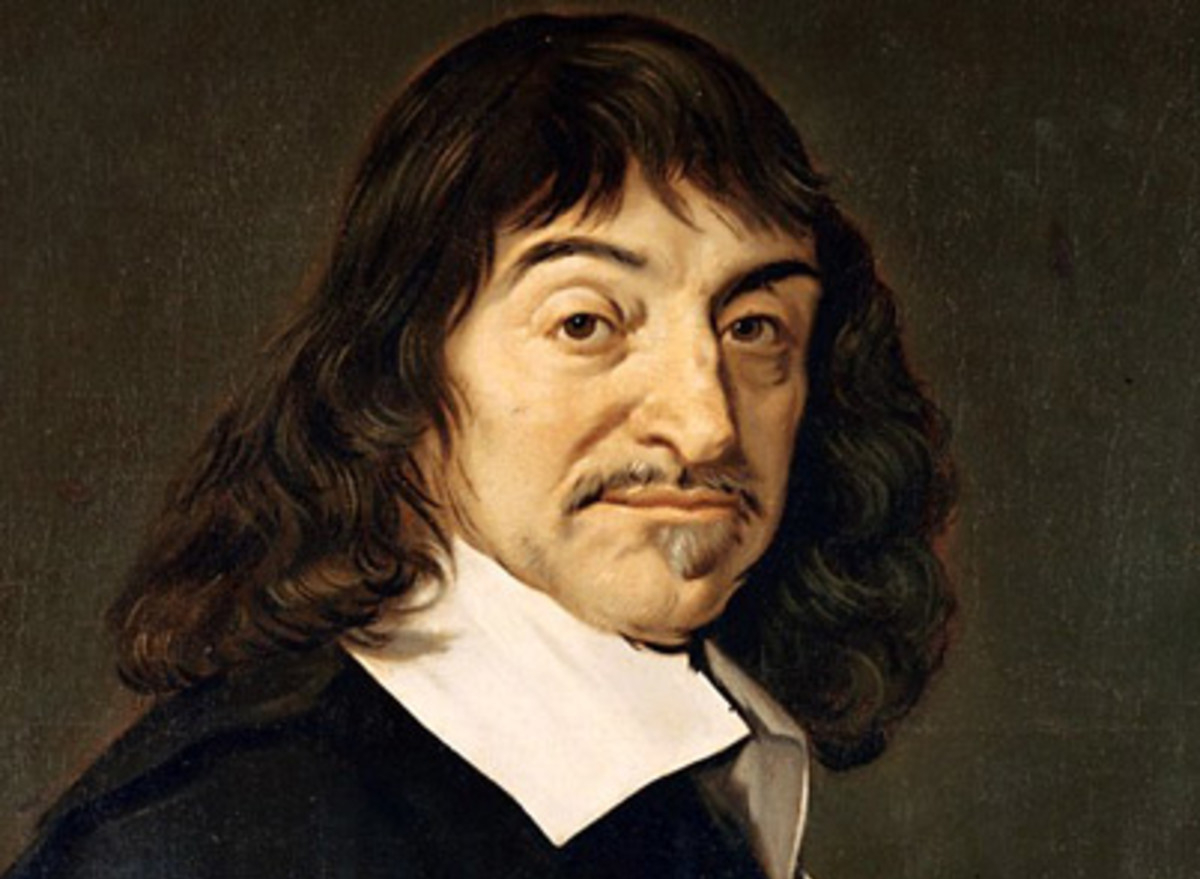
\includegraphics[width=14cm]{../resources/jpg/2.3.functions/descartes.jpg}
    \caption*{Rene Descartes.}
\end{figure}
\subsection[The composition of surjective functions is surjective.]
    {
        \color{section}Theorem 67. \color{black} The composition of surjective functions.
    }
\documentclass[preview]{standalone}
\usepackage{amssymb, amsthm}
\usepackage{mathtools}
\usepackage{bm}


\newtheorem{theorem}{Theorem}
\renewcommand\qedsymbol{$\blacksquare$}


\begin{document}


\begin{theorem}[\textbf{2329b}]
    Let \bm{$\delta$} be a function 
    \bm{$\delta: \Delta \rightarrow \mathrm{A}$}, 
    and let \bm{$\gamma$} be a function 
    \bm{$\gamma : \Lambda \rightarrow \Delta$}. 
    \begin{center}
        If both \bm{$\delta$} and \bm{$\gamma$} are surjective, 
        then 
        \bm{$\big \langle \delta \circ \gamma \big \rangle$} 
        is surjective.
    \end{center}
\end{theorem}

\begin{proof}
    By the contrapositive. 
    Suppose it were not the case that
    \bm{$\big \langle \delta \circ \gamma \big \rangle$} 
    were surjective. 
    By the definition for surjective functions,
    with domain of discourse \bm{$\lambda \in \Lambda$} 
    and \bm{$\alpha \in \mathrm{A}$}, 
    that is
    \begin{equation*}
        \lnot \forall \alpha \exists \lambda \Big \langle
            \big \langle \delta \circ \gamma \big \rangle [\lambda] 
                = 
            \alpha
        \Big \rangle
    \end{equation*}
    The composition of functions 
    \bm{$\big \langle \delta \circ \gamma \big \rangle [\lambda]$} 
    is defined as \bm{$\delta \big[ \gamma(\lambda) \big]$}.
    Thus, we have the equivalent universal quantification
    \begin{equation*}
        \lnot \forall \alpha \exists \lambda \Big \langle
            \delta \big[ \gamma (\lambda) \big] = \alpha \Big \rangle
    \end{equation*}
    In other words, it follows from the negation of the direct consequent 
    that it is not the case that \bm{$\delta$} is surjective, 
    by the definition for surjective functions.
    This is sufficient to prove the logical negation of the direct hypothesis.
    Thus, if both \bm{$\delta$} and \bm{$\gamma$} are surjective, 
    then \bm{$\big \langle \delta \circ \gamma \big \rangle$} is surjective.
\end{proof}


\end{document}
\pagebreak


% ============================== 0068 Theorem 2330 ================================
\begin{figure}[!h]
    \centering
    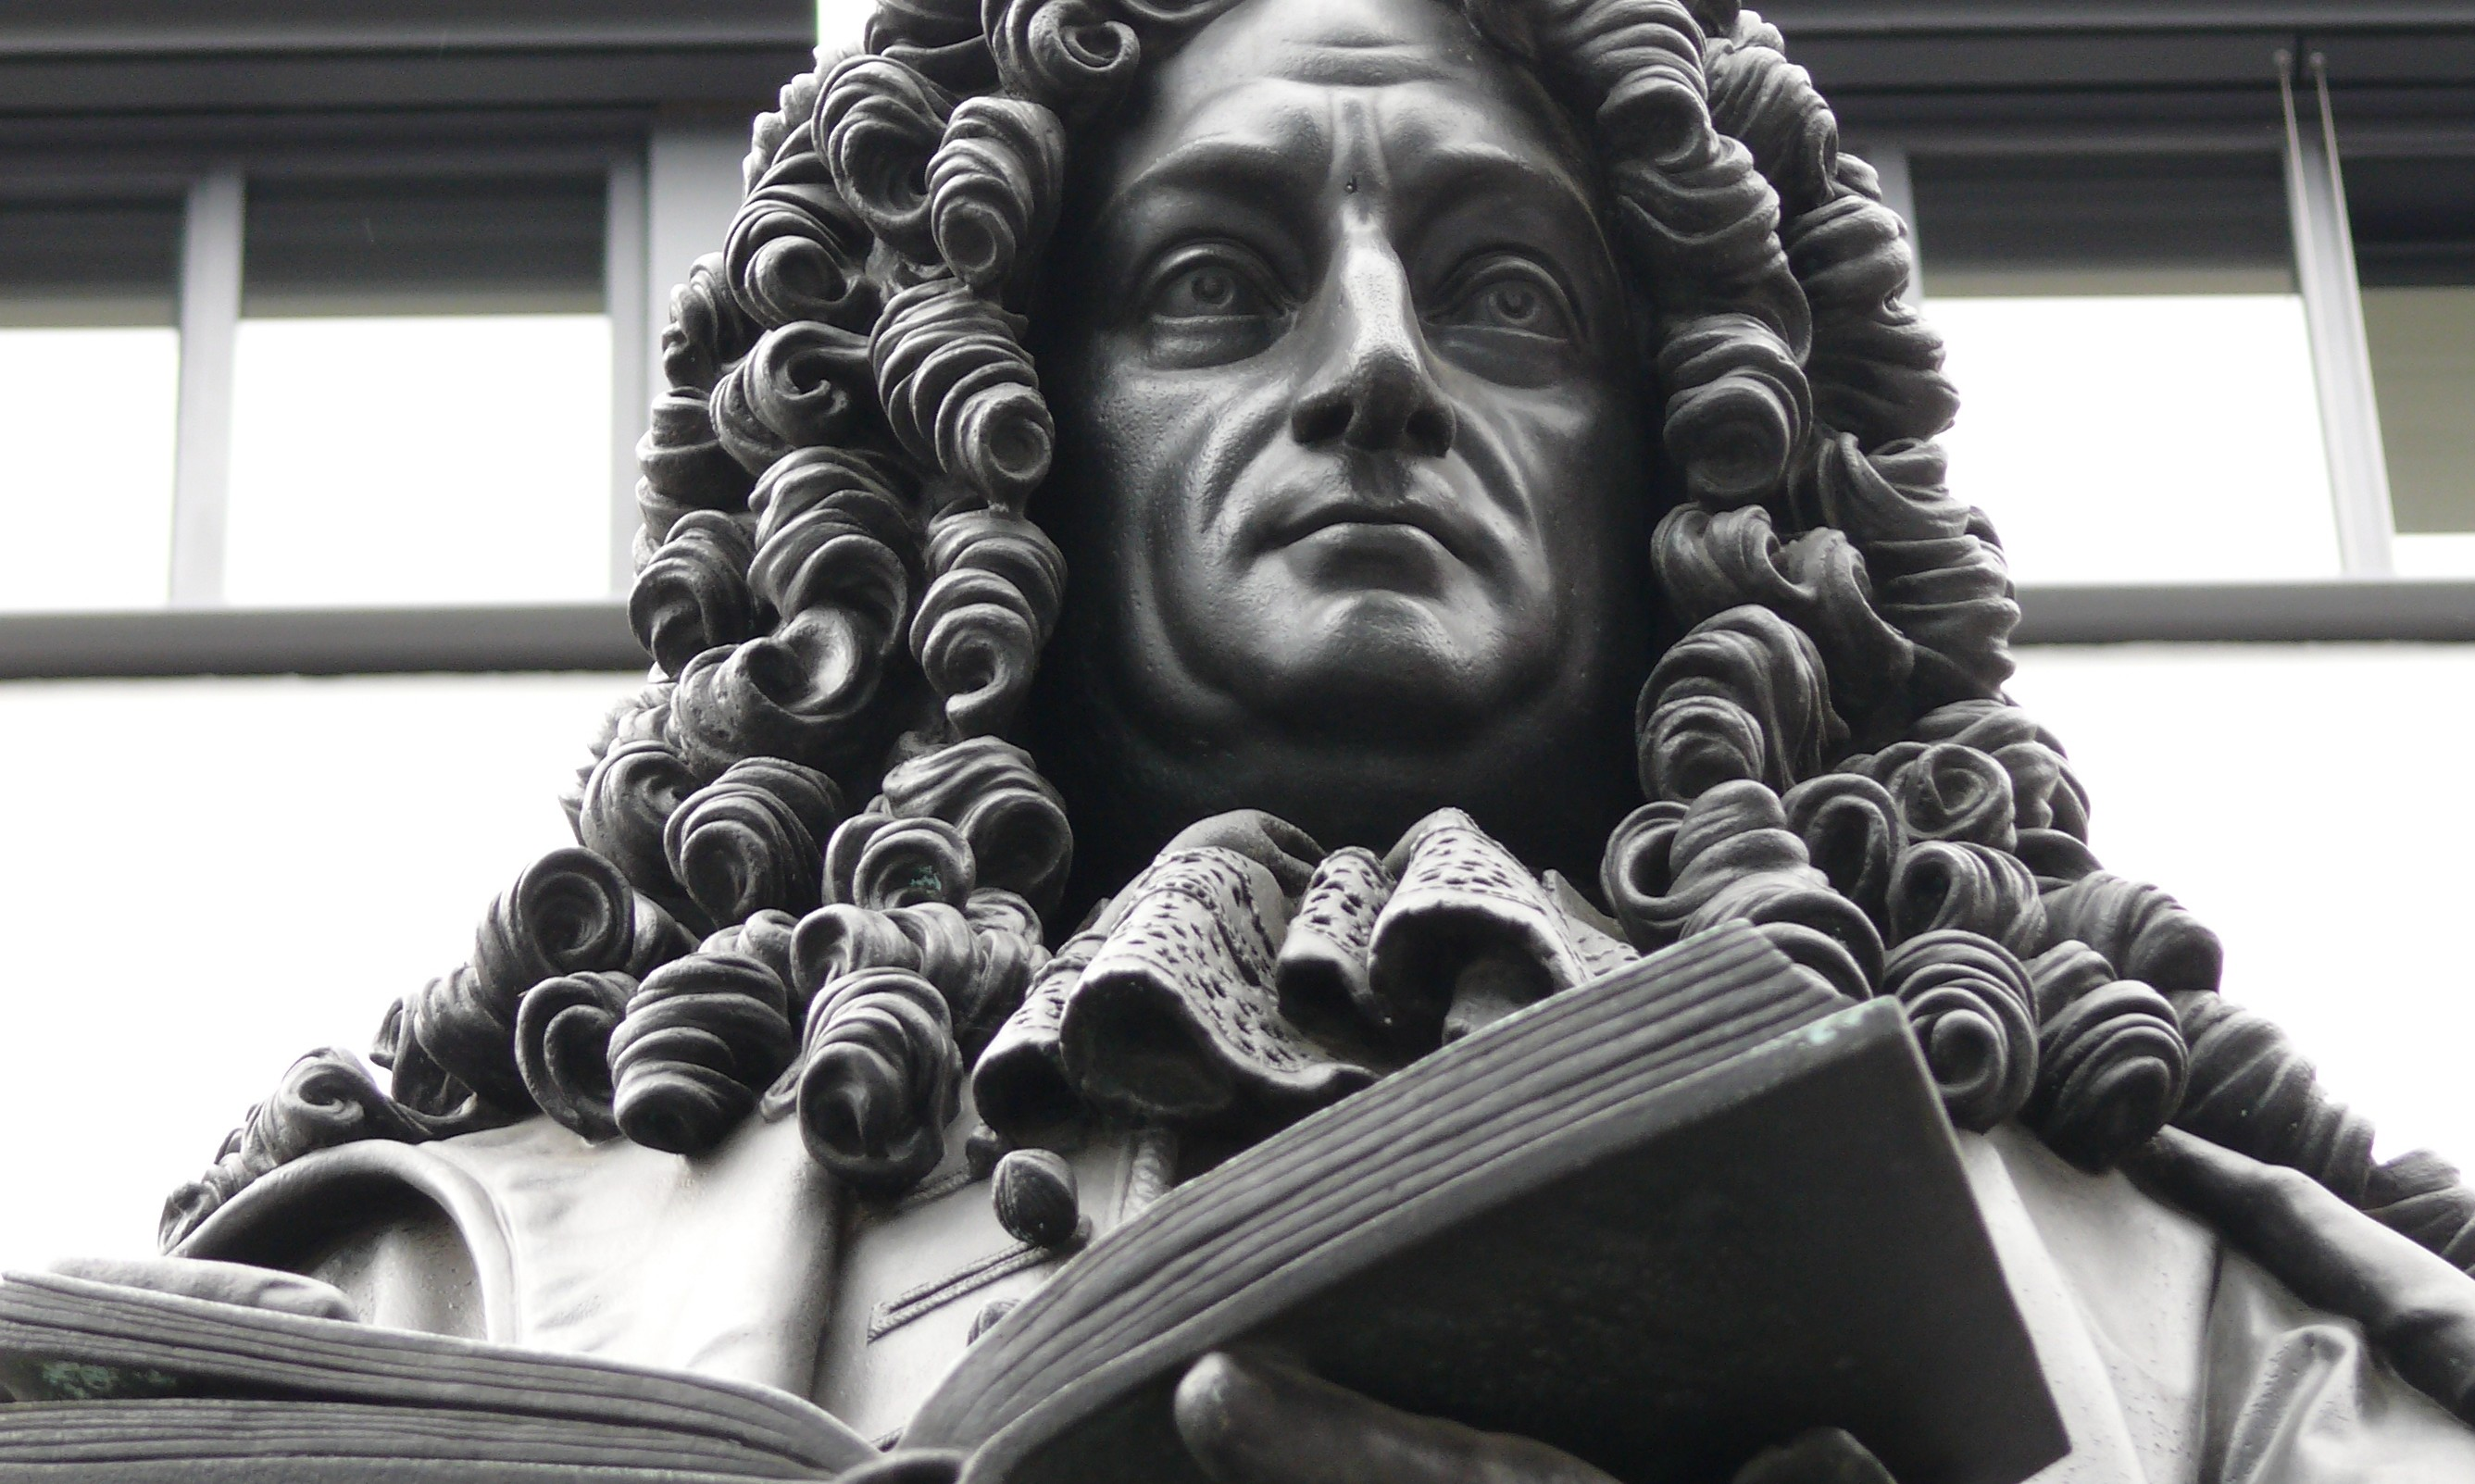
\includegraphics[width=14cm]{../resources/jpg/2.3.functions/leibniz.jpg}
    \caption*{Gottfried Wilhelm Leibniz.}
\end{figure}
\subsection[The subject function in an injective composition is injective.]
    {
        \color{section}Theorem 68. \color{black} The subject in an injective composition.
    }
\documentclass[preview]{standalone}
\usepackage{amssymb, amsthm}
\usepackage{mathtools}
\usepackage{bm}


\newtheorem{theorem}{Theorem}
\renewcommand\qedsymbol{$\blacksquare$}


\begin{document}


\begin{theorem}[\textbf{2330}]
    Let \bm{$\delta$} and 
    \bm{$\big \langle \delta \circ \gamma \big \rangle$} 
    be injective functions.
    \bm{$\gamma$} is injective.
\end{theorem}

\begin{proof}
    By the contrapositive. Suppose that \bm{$\gamma$} were not injective. 
    Then by the definition for injective functions we have the following universally quantified statement, 
    with the domain of discourse being the domain of \bm{$\gamma$},
    \begin{equation*}
        \lnot \forall \mu \forall \nu \Big \langle
            \big \langle \gamma [\mu] = \gamma [\nu] \big \rangle
                \rightarrow 
            \big \langle \mu = \nu \big \rangle
        \Big \rangle
    \end{equation*}
    By the equality properties for equations, and by the defintion for the composition of functions,
    \begin{equation*}
        \Big \langle
            \gamma[\mu] = \gamma[\nu] 
        \Big \rangle
            \rightarrow 
        \bigg\{
            \Big \langle
                \delta \big[ \gamma(\mu) \big] 
                    = 
                \delta \big[ \gamma(\nu) \big] 
            \Big \rangle
                \equiv 
            \Big[
                \big \langle \delta \circ \gamma \big \rangle [\mu] 
                    = 
                \big \langle \delta \circ \gamma \big \rangle [\nu]
            \Big]
        \bigg\}
    \end{equation*}
    Thus, the universal quantification above implies
    \begin{equation*}
        \lnot \forall \mu \forall \nu \bigg \langle
            \Big\{
                \big \langle \delta \circ \gamma \big \rangle [\mu] 
                    = 
                \big \langle \delta \circ \gamma \big \rangle [\nu]
            \Big\}
                \rightarrow
            \big \langle \mu = \nu \big \rangle
        \bigg \rangle
    \end{equation*}
    That is, 
    it is not the case that 
    \bm{$\big \langle \delta \circ \gamma \big \rangle$} is injective, by the definition for injective functions. 
    Since it follows directly from the negation of the consequent that 
    \bm{$\big \langle \delta \circ \gamma \big \rangle$} is not injective:
    if \bm{$\delta$} and 
    \bm{$\big \langle \delta \circ \gamma \big \rangle$} 
    are injective functions, 
    then \bm{$\gamma$} is indeed injective.
\end{proof}


\end{document}
\pagebreak


% ============================== 0069 Theorem 2336a ===============================
\subsection[The image of a union under the function lambda.]
    {
        \color{section}Theorem 69. \color{black} The image of a union under lambda.
    }
\documentclass[preview]{standalone}
\usepackage{amssymb, amsthm}
\usepackage{mathtools}
\usepackage{bm}


\newtheorem{theorem}{Theorem}
\renewcommand\qedsymbol{$\blacksquare$}


\begin{document}


\begin{theorem}[\textbf{2336a}]
    Let \bm{$\lambda$} be the function 
    \bm{$\lambda: \Gamma \to \Phi$}. 
    Let \bm{$\mathrm{A}$}, and \bm{$\Lambda$} be subsets of \bm{$\Gamma$}. 
    \begin{equation*}
        \bm{
            \lambda \big[ \mathrm{A} \cup \Lambda \big] 
                = 
            \lambda \big[ \mathrm{A} \big] \cup \lambda \big[ \Lambda \big]
        }
    \end{equation*}
\end{theorem}

\begin{proof}
    Suppose there exists an element \bm{$\phi$} such that
    \bm{$\phi \in \lambda \big[ \mathrm{A} \cup \Lambda \big]$}.
    By the definition for the image of a set under the function \bm{$\lambda$},
    \bm{$\phi = \lambda \big[ \iota \big]$} 
    where \bm{$\iota$} is an element in \bm{$\mathrm{A} \cup \Lambda$}. 
    That is, by the definition for the union of sets,
    \bm{$\iota \in \mathrm{A} \lor \iota \in \Lambda$}. 
    Thus, 
    \bm{$\phi \in \lambda \big[ \mathrm{A} \big] \lor \phi \in \lambda \big[ \Lambda \big]$}.
    And by the definition for set union, 
    \bm{$\phi \in \lambda \big[ \mathrm{A} \big] \cup \lambda \big[ \Lambda \big]$}.
    
    Suppose there exists an element \bm{$\phi$} such that 
    \bm{$\phi \in \lambda \big[ \mathrm{A} \big] \cup \lambda \big[ \Lambda \big]$}.
    By the defintion for set union, 
    \bm{$\phi \in \lambda \big[ \mathrm{A} \big] \lor \phi \in \lambda \big[ \Lambda \big]$}.
    By the definition for the image of a set under the function \bm{$\lambda$},
    there exists an element \bm{$\iota \in \mathrm{A} \lor \iota \in \Lambda$} such that 
    \bm{$\lambda \big[ \iota \big] = \phi$}.
    By the definition for set union, 
    \bm{$\iota \in \mathrm{A} \cup \Lambda$}.
    Hence,
    \bm{$\phi \in \lambda \big[ \mathrm{A} \cup \Lambda \big]$}
\end{proof}


\end{document}
\sep


% ============================== 0070 Theorem 2336b ===============================
\subsection[The image of an intersection under lambda.]
    {
        \color{section}Theorem 70. \color{black} The image of an intersection.
    }
\documentclass[preview]{standalone}
\usepackage{amssymb, amsthm}
\usepackage{mathtools}
\usepackage{bm}


\newtheorem{theorem}{Theorem}
\renewcommand\qedsymbol{$\blacksquare$}


\begin{document}


\begin{theorem}[\textbf{2236b}]
    Let \bm{$\lambda$} be the function 
    \bm{$\lambda : \Gamma \rightarrow \Delta$}. 
    Let \bm{$\mathrm{A}$}, 
    and \bm{$\Lambda$} be subsets of \bm{$\Gamma$}.
    \begin{equation*}
        \bm{
            \Big \langle \lambda \big[ \mathrm{A} \cap \Lambda \big] \Big \rangle
                \subseteq 
            \Big \langle \lambda \big[ \mathrm{A} \big] \cap \lambda \big[ \Lambda \big] \Big \rangle
        }
    \end{equation*}
\end{theorem}

\begin{proof}
    Let \bm{$\iota$} be an element in \bm{$\Gamma$} such that 
    \bm{$\lambda \big[ \iota \big]$} is a member of 
    \bm{$\lambda \big[ \mathrm{A} \cap \Lambda \big]$}. 
    By the definition for the image of 
    \bm{$\big \langle \mathrm{A} \cap \Lambda \big \rangle$} 
    under the function \bm{$\lambda$}, 
    \bm{$\iota$} is an element in 
    \bm{$\big \langle \mathrm{A} \cap \Lambda \big \rangle$}. 
    By the definition for the
    intersection of sets 
    \begin{equation*}
        \Big \langle \iota \in \mathrm{A} \Big \rangle 
            \land 
        \Big \langle \iota \in \Lambda \Big \rangle
    \end{equation*}
    Thus,
    \begin{equation*}
        \Big \langle 
            \lambda \big[ \iota \big] 
                \in 
            \lambda \big[ \mathrm{A} \big]
        \Big \rangle 
            \land 
        \Big \langle
            \lambda \big[ \iota \big] 
                \in 
            \lambda \big[ \Lambda \big]
        \Big \rangle
    \end{equation*} 
    By the definition for set intersection,
    \bm{$\lambda \big[ \iota \big]$} is a member of
    \bm{$
        \big \langle 
            \lambda \big[ \mathrm{A} \big] 
                \cap 
            \lambda \big[ \Lambda \big]
        \big \rangle    
    $},
    $\therefore \text{\space} \bm{
        \lambda \big[ \mathrm{A} \cap \Lambda \big] 
            \subseteq 
        \lambda \big[ \mathrm{A} \big] \cap \lambda \big[ \Lambda \big]
    }$.
\end{proof}


\end{document}
\pagebreak


% ============================== 0071 Theorem 2340a ===============================
\subsection[The inverse image of a union under lambda.]
    {
        \color{section}Theorem 71. \color{black} The inverse image of a union.
    }
\documentclass[preview]{standalone}
\usepackage{amssymb, amsthm}
\usepackage{mathtools}
\usepackage{bm}


\newtheorem{theorem}{Theorem}
\renewcommand\qedsymbol{$\blacksquare$}


\begin{document}


\begin{theorem}[\textbf{2340a}]
    Let \bm{$\lambda$} be the function 
    \bm{$\lambda : \Gamma \rightarrow \mathrm{A}$}. 
    Let \bm{$\Lambda$}, and \bm{$\Delta$} 
    be subsets of \bm{$\mathrm{A}$}.
    \begin{equation*}
        \bm{
        \lambda ^{-1} \big[ \Lambda \cup \Delta \big] 
            = 
        \lambda ^{-1} 
            \big[ \Lambda \big] 
                \cup 
            \lambda^{-1} \big[ \Delta \big]
        }
    \end{equation*}
\end{theorem}

\begin{proof}
    Let \bm{$\iota$} be an element in \bm{$\lambda ^{-1} \big[ \Lambda \cup \Delta \big]$}.
    By the inverse function for
    \bm{$\lambda ^{-1}$}, 
    and by the definition for the union of sets, that is 
    \begin{equation*}
        \bigg \langle \lambda 
            \big[ \iota \big] 
                \in 
            \lambda \Big[ 
                \lambda ^{-1} \big[ \Lambda \cup \Delta \big]
            \Big]
        \bigg \rangle
            \equiv
        \bigg[
            \Big \langle \lambda \big[ \iota \big] \in \Lambda \Big \rangle
                \lor 
            \Big \langle \lambda \big[ \iota \big] \in \Delta \Big \rangle
        \bigg]
    \end{equation*}
    By \bm{$\lambda$} inverse, and by the definition for set union, that is
    \begin{equation*}
        \bigg[
            \Big \langle
                \iota \in \lambda^{-1} \big[ \Lambda \big] 
            \Big \rangle
                \lor 
            \Big \langle
                \iota \in \lambda^{-1} \big[ \Delta \big]
            \Big \rangle
        \bigg]
            \equiv
        \bigg[ 
            \iota \in \Big \langle
                \lambda ^{-1} \big[ \Lambda \big] 
                    \cup 
                \lambda ^{-1} \big[ \Delta \big]
            \Big \rangle
        \bigg]
    \end{equation*}
    $\therefore \text{\space} \bm{
    \lambda ^{-1} \big[ \Lambda \cup \Delta \big] 
        = 
    \lambda ^{-1} 
        \big[ \Lambda \big] 
            \cup 
        \lambda^{-1} \big[ \Delta \big]
    }$.
\end{proof}


\end{document}
\sep


% ============================== 0072 Theorem 2340b ===============================
\subsection[The inverse image of an intersection under lambda.]
    {
        \color{section}Theorem 72. \color{black} The inverse image of an intersection.
    }
\documentclass[preview]{standalone}
\usepackage{amssymb, amsthm}
\usepackage{mathtools}
\usepackage{bm}


\newtheorem{theorem}{Theorem}
\renewcommand\qedsymbol{$\blacksquare$}


\begin{document}


\begin{theorem}[\textbf{2340b}]
    Let \bm{$\lambda$} be the function 
    \bm{$\lambda : \Gamma \rightarrow \mathrm{A}$}. 
    Let \bm{$\Lambda$}, and \bm{$\Delta$} 
    be subsets of \bm{$\mathrm{A}$}. 
    \begin{equation*}
        \bm{
        \lambda ^{-1} \big[ \Lambda \cap \Delta \big] 
            = 
        \lambda ^{-1} 
            \big[ \Lambda \big] 
                \cap 
            \lambda^{-1} \big[ \Delta \big]
        }
    \end{equation*}
\end{theorem}

\begin{proof}
    Let \bm{$\iota$} be an element in \bm{$\lambda ^{-1} \big[ \Lambda \cap \Delta \big]$}.
    By the inverse function for
    \bm{$\lambda ^{-1}$}, 
    and by the definition for the intersection of sets, that is 
    \begin{equation*}
        \bigg \langle \lambda 
            \big[ \iota \big] 
                \in 
            \lambda \Big[ 
                \lambda ^{-1} \big[ \Lambda \cap \Delta \big]
            \Big]
        \bigg \rangle
            \equiv
        \bigg[
            \Big \langle \lambda \big[ \iota \big] \in \Lambda \Big \rangle
                \land 
            \Big \langle \lambda \big[ \iota \big] \in \Delta \Big \rangle
        \bigg]
    \end{equation*}
    By \bm{$\lambda$} inverse, and by the definition for set intersection, that is
    \begin{equation*}
        \bigg[
            \Big \langle
                \iota \in \lambda^{-1} \big[ \Lambda \big] 
            \Big \rangle
                \land 
            \Big \langle
                \iota \in \lambda^{-1} \big[ \Delta \big]
            \Big \rangle
        \bigg]
            \equiv
        \bigg[ 
            \iota \in \Big \langle
                \lambda ^{-1} \big[ \Lambda \big] 
                    \cap 
                \lambda ^{-1} \big[ \Delta \big]
            \Big \rangle
        \bigg]
    \end{equation*}
    $\therefore \text{\space} \bm{
    \lambda ^{-1} \big[ \Lambda \cap \Delta \big] 
        = 
    \lambda ^{-1} 
        \big[ \Lambda \big] 
            \cap 
        \lambda^{-1} \big[ \Delta \big]
    }$.
\end{proof}


\end{document}
\pagebreak


% ============================== 0073 Theorem 2341 ================================
\begin{figure}[!h]
    \centering
    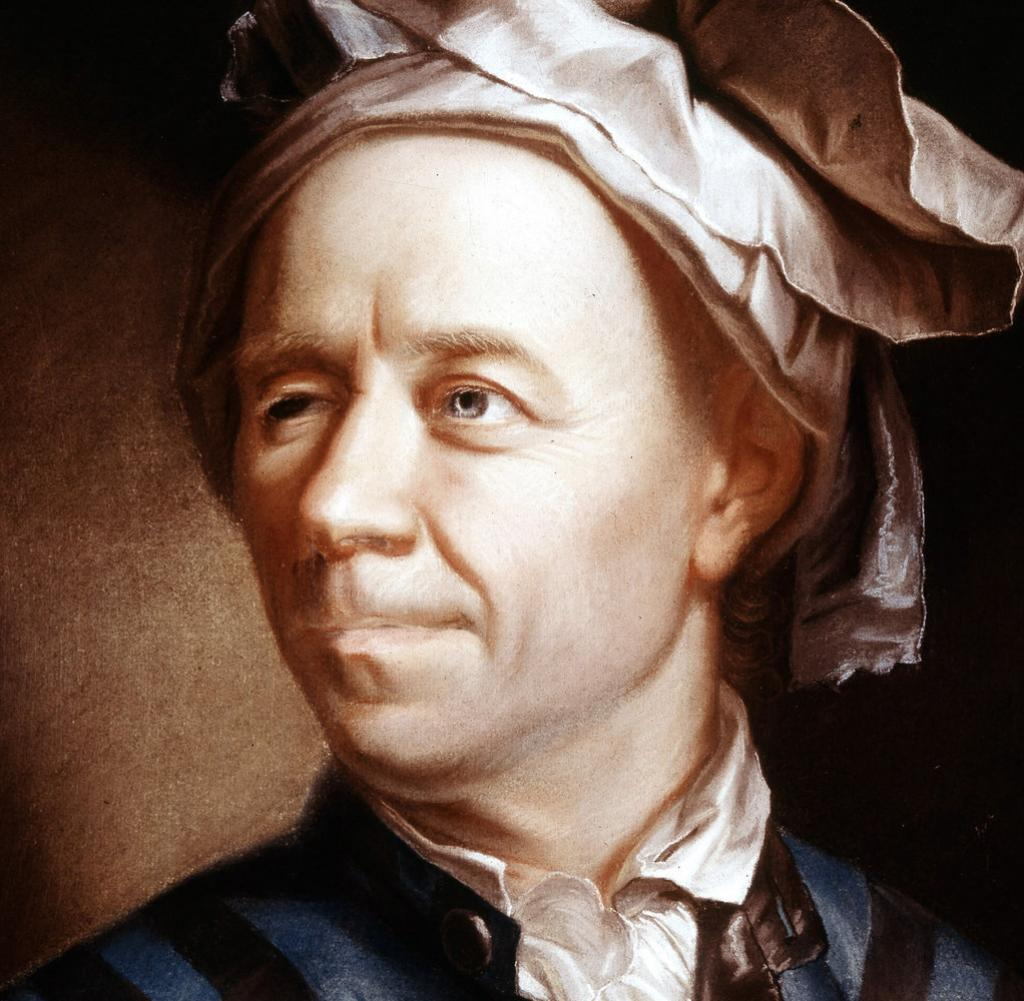
\includegraphics[width=14cm]{../resources/jpg/2.3.functions/euler.jpg}
    \caption*{Leonard Euler.}
\end{figure}
\subsection[The inverse image of a complement under lambda.]
    {
        \color{section}Theorem 73. \color{black} The inverse image of a complement.
    }
\documentclass[preview]{standalone}
\usepackage{amssymb, amsthm}
\usepackage{mathtools}
\usepackage{bm}


\newtheorem{theorem}{Theorem}
\renewcommand\qedsymbol{$\blacksquare$}


\begin{document}


\begin{theorem}[\textbf{2341}]
    Let \bm{$\lambda$} be the function 
    \bm{$\lambda : \Delta \rightarrow \mathrm{A}$}. 
    Let \bm{$\Lambda$} be a subset of \bm{$\mathrm{A}$}. 
    \begin{equation*}
        \bm{
        \lambda ^{-1} \big[ \overline{\Lambda} \big] 
            = 
        \overline{ \lambda ^{-1} \big[ \Lambda \big]}
        }
    \end{equation*}
\end{theorem}

\begin{proof}
    Let \bm{$\alpha$} be an element in 
    \bm{$\lambda ^{-1} \big[ \overline{\Lambda} \big]$}.
    By \bm{$\lambda ^{-1}$} inverse, by the definition of set complement,
    by \bm{$\lambda$} inverse, and again by the defintion of set complement,
    \begin{equation*}
        \Big \langle
            \alpha \in \lambda ^{-1} \big[ \overline{\Lambda} \big]
        \Big \rangle
            \equiv
        \Big \langle
            \lambda \big[ \alpha \big] \in \overline{\Lambda}
        \Big \rangle
            \equiv
        \Big \langle
            \lambda \big[ \alpha \big] \notin \Lambda
        \Big \rangle
            \equiv
    \end{equation*}
    \begin{equation*}
        \Big \langle 
            \alpha 
                \notin 
            \lambda ^{-1} \big[ \Lambda \big]
        \Big \rangle
            \equiv
        \Big \langle
            \alpha 
                \in
            \overline{
                \lambda ^{-1} \big[ \Lambda \big]
            }
        \Big \rangle
    \end{equation*}
    $\therefore \text{\space} \bm{
        \lambda ^{-1} \big[ \overline{\Lambda} \big] 
            = 
        \overline{ \lambda ^{-1} \big[ \Lambda \big]}
    }$.
\end{proof}


\end{document}
\pagebreak


% ============================== 0074 Theorem 2342 ================================
\subsection[The floor of zeta plus one half.]
    {
        \color{section}Theorem 74. \color{black} The floor of zeta plus one half.
    }
\documentclass[preview]{standalone}
\usepackage{amssymb, amsthm}
\usepackage{mathtools}
\usepackage{bm}


\newtheorem{theorem}{Theorem}
\renewcommand\qedsymbol{$\blacksquare$}


\begin{document}


\begin{theorem}[\textbf{2342}]
    Let \bm{$\zeta$} be a real number.
    \begin{center}
        \bm{$\lfloor \zeta + \frac{1}{2} \rfloor$}
        is the closest integer to \bm{$\zeta$}, 
        except when \bm{$\zeta$} is midway between two integers, 
        when it is the larger of these two integers.
    \end{center}
\end{theorem}

\begin{proof}
    By cases. By the properties of floor functions, 
    there exists an integer \bm{$\lambda$} such that 
    \begin{equation*}
        \Big \langle \lambda \Big \rangle
            \le 
        \Big \langle \zeta \Big \rangle
            < 
        \Big \langle \lambda + 1 \Big \rangle
    \end{equation*}
    and 
    \bm{$\zeta - \lfloor \zeta \rfloor = \epsilon$}.
    \\ \\
    \bm{$(i)$} Suppose the case in which \bm{$\zeta$} is midway between two integers, 
    or is closest to the larger of two integers \bm{$\lambda$} and 
    \bm{$\big \langle \lambda + 1 \big \rangle$}. 
    Then, the inequality \bm{$\frac{1}{2} \leq \epsilon < 1$} must be true. Thus, 
    \begin{equation*}
        \bigg[
            \Big \langle
                \lambda + \frac{1}{2}
            \Big \rangle
                \leq 
            \Big \langle
                \lambda + \epsilon
            \Big \rangle
                <
            \Big \langle
                \lambda + 1
            \Big \rangle
        \bigg]
            \equiv
        \bigg[
            \Big \langle    
                \lambda + \frac{1}{2}
            \Big \rangle
                \leq
            \Big \langle
                \zeta
            \Big \rangle
                <
            \Big \langle
                \lambda + 1
            \Big \rangle
        \bigg]
            \equiv
    \end{equation*}
    \begin{equation*}
        \bigg[
            \Big \langle 
                \lambda + 1
            \Big \rangle
                \leq
            \Big \langle 
                \zeta + \frac{1}{2}
            \Big \rangle
                <
            \Big \langle
                \lambda + 1 + \frac{1}{2}
            \Big \rangle
        \bigg]
    \end{equation*}
    Since 
    \bm{$
    \big \langle \lambda + 1 + \frac{1}{2} \big \rangle 
        < 
    \big \langle 
        \lambda + 1 + 1
    \big \rangle
    $}, 
    the integer \bm{$\lfloor \zeta + \frac{1}{2} \rfloor$} is 
    \bm{$\big \langle \lambda + 1 \big \rangle$}, 
    by the properties for floor functions,
    and by the law of transitivity from the order axioms.
    \\ \\
    \bm{$(ii)$} Suppose the case in which \bm{$\zeta$} is closest to the integer \bm{$\lambda$}. 
    Then the inequality \bm{$0 \leq \epsilon < \frac{1}{2}$}, 
    must be true. Thus, 
    \begin{equation*}
        \bigg[
            \Big \langle
                \lambda + 0
            \Big \rangle
                \leq
            \Big \langle
                \lambda + \epsilon
            \Big \rangle
                <
            \Big \langle
                \lambda + \frac{1}{2}
            \Big \rangle
        \bigg]
            \equiv
    \end{equation*}
    \begin{equation*}
        \bigg[
            \Big \langle
                \lambda
            \Big \rangle
                \leq
            \Big \langle
                \zeta
            \Big \rangle
                <
            \Big \langle
                \lambda + \frac{1}{2}
            \Big \rangle
        \bigg]
            \equiv
        \bigg[
            \Big \langle
                \lambda + \frac{1}{2}
            \Big \rangle
                \leq
            \Big \langle
                \zeta + \frac{1}{2}
            \Big \rangle
                <
            \Big \langle
                \lambda + 1
            \Big \rangle
        \bigg]
    \end{equation*}
    Since 
    \bm{$
    \big \langle \lambda \big \rangle 
        \leq 
    \big \langle \lambda + \frac{1}{2} \big \rangle
    $},
    the integer \bm{$\lfloor \zeta + \frac{1}{2} \rfloor$} is 
    \bm{$\big \langle \lambda \big \rangle$}, 
    by the properties for floor functions,
    and by the law of transitivity from the order axioms.
    $\therefore$
    \bm{$\lfloor \zeta + \frac{1}{2} \rfloor$} 
    is the closest integer to \bm{$\zeta$}, 
    except when \bm{$\zeta$} is midway between two integers, 
    when it is the larger of these two integers.
\end{proof}


\end{document}
\begin{figure}[!h]
    \centering
    
\includegraphics[width=2.5cm]{../resources/jpg/2.3.functions/symbol1.jpg}
\end{figure}
\pagebreak


% ============================== 0075 Theorem 2343 ================================
\subsection[The ceiling of zeta minus one half.]
    {
        \color{section}Theorem 75. \color{black} The ceiling of zeta minus one half.
    }
\documentclass[preview]{standalone}
\usepackage{amssymb, amsthm}
\usepackage{mathtools}
\usepackage{bm}


\newtheorem{theorem}{Theorem}
\renewcommand\qedsymbol{$\blacksquare$}


\begin{document}


\begin{theorem}[\textbf{2343}]
    Let \bm{$\zeta$} be a real number. 
    \begin{center}
        \bm{$\lceil \zeta - \frac{1}{2} \rceil$} is the closest integer to \bm{$\zeta$}, 
        except when \bm{$\zeta$} is midway between two integers, 
        when it is the smaller of these two integers.
    \end{center}
\end{theorem}

\begin{proof}
    By cases. By the properties of ceiling functions, 
    there exists an integer \bm{$\lambda$} such that 
    \begin{equation*}
        \Big \langle \lambda - 1 \Big \rangle
            < 
        \Big \langle \zeta \Big \rangle
            \leq 
        \Big \langle \lambda \Big \rangle
    \end{equation*}
    and 
    \bm{$\lceil \zeta \rceil - \zeta = \epsilon$}. 
    \\ \\
    \bm{$(i)$} Suppose the case in which 
    \bm{$\zeta$} is midway between two integers, 
    or is closest to the smaller of two integers 
    \bm{$\big \langle \lambda -1 \big \rangle$} and
    \bm{$\lambda$}. 
    Then, the inequality,
    \bm{$1 > \epsilon \geq \frac{1}{2}$} 
    must be true. Thus, 
    \begin{equation*}
        \bigg[
            \Big \langle
                \lambda - 1
            \Big \rangle
                <
            \Big \langle
                \lambda - \epsilon
            \Big \rangle
                \leq
            \Big \langle
                \lambda - \frac{1}{2}
            \Big \rangle
        \bigg]
            \equiv
        \bigg[
            \Big \langle
                \lambda - 1
            \Big \rangle
                <
            \Big \langle
                \zeta
            \Big \rangle
                \leq
            \Big \langle    
                \lambda - \frac{1}{2}
            \Big \rangle
        \bigg]
            \equiv
    \end{equation*}
    \begin{equation*}
        \bigg[
            \Big \langle
                \lambda - 1 - \frac{1}{2}
            \Big \rangle
                <
            \Big \langle 
                \zeta - \frac{1}{2}
            \Big \rangle
                \leq
            \Big \langle 
                \lambda - 1
            \Big \rangle
        \bigg]
    \end{equation*}
    Since 
    \bm{$
    \big \langle \lambda - 1 - 1 \big \rangle 
        < 
    \big \langle \lambda - 1 - \frac{1}{2} \big \rangle
    $},
    the integer \bm{$\lceil \zeta - \frac{1}{2} \rceil$} is 
    \bm{$\big \langle \lambda - 1 \big \rangle$}, 
    by the properties for ceiling functions,
    and by the law of transitivity from the order axioms.
    \\ \\
    \bm{$(ii)$} Suppose the case in which 
    \bm{$\zeta$} is closest to the integer \bm{$\lambda$}. 
    Then, the inequality 
    \bm{$\frac{1}{2} > \epsilon \geq 0$}
    must be true. Thus, 
    \begin{equation*}
        \bigg[
            \Big \langle
                \lambda - \frac{1}{2}
            \Big \rangle
                <
            \Big \langle
                \lambda - \epsilon
            \Big \rangle
                \leq
            \Big \langle
                \lambda - 0
            \Big \rangle
        \bigg]
            \equiv
    \end{equation*}
    \begin{equation*}
        \bigg[
            \Big \langle
                \lambda - \frac{1}{2}
            \Big \rangle
                <
            \Big \langle
                \zeta
            \Big \rangle
                \leq
            \Big \langle
                \lambda
            \Big \rangle
        \bigg]
            \equiv
        \bigg[
            \Big \langle
                \lambda - 1
            \Big \rangle
                <
            \Big \langle
                \zeta - \frac{1}{2}
            \Big \rangle
                \leq
            \Big \langle
                \lambda - \frac{1}{2}
            \Big \rangle
        \bigg]
    \end{equation*}
    Since 
    \bm{$
    \big \langle \lambda - \frac{1}{2} \big \rangle 
        \leq
    \big \langle 
        \lambda
    \big \rangle
    $}, 
    the integer \bm{$\lceil \zeta - \frac{1}{2} \rceil$} is 
    \bm{$\big \langle \lambda \big \rangle$}, 
    by the properties for ceiling functions,
    and by the law of transitivity from the order axioms
    $\therefore \text{\space} \bm{
    \lceil \zeta - \frac{1}{2} \rceil}$ 
    is the closest integer to \bm{$\zeta$}, 
    except when \bm{$\zeta$} is midway between two integers, 
    when it is the smaller of these two integers.
\end{proof}


\end{document}
\vspace{.25\baselineskip}
\sep
\pagebreak


% ============================== 0076 Theorem 2344 ================================
\subsection[The difference between a ceiling and a floor.]
    {
        \color{section}Theorem 76. \color{black} The difference between ceiling and floor.
    }
\documentclass[preview]{standalone}
\usepackage{amssymb, amsthm}
\usepackage{mathtools}
\usepackage{bm}


\newtheorem{theorem}{Theorem}
\renewcommand\qedsymbol{$\blacksquare$}


\begin{document}


\begin{theorem}[\textbf{2344}]
    Let \bm{$\lambda$} be a real number.
    \begin{equation*}
        \bm{\lceil \lambda \rceil 
            - 
        \lfloor \lambda \rfloor 
            = 
        1
            \textbf{, if }
        \lambda \notin \mathbb{Z} 
            \textbf{. }
        \lceil \lambda \rceil
            - 
        \lfloor \lambda \rfloor 
            = 
        0
            \textbf{, if }
        \lambda \in \mathbb{Z}}
    \end{equation*} 
\end{theorem}

\begin{proof}
    Let \bm{$\lambda - \lfloor \lambda \rfloor = \sigma$}.
    By the properties for ceiling functions,
    there exists an integer \bm{$\zeta$} such that
    \bm{$\lceil \lambda \rceil = \zeta$}, 
    if and only if
    \begin{equation*}
        \Big \langle \zeta - 1 \Big \rangle
            < 
        \Big \langle \lambda \Big \rangle
            \leq 
        \Big \langle \zeta \Big \rangle
    \end{equation*}
    By the identity of \bm{$\zeta$}, 
    and by the additive compatibility law from the order axioms
    (subtracting \bm{$\lfloor \lambda \rfloor$} from every side,)
    that is,
    \begin{equation*}
        \Big \langle \lceil \lambda \rceil - 1 \Big \rangle 
            <
        \Big \langle \lambda \Big \rangle
            \leq 
        \Big \langle \lceil \lambda \rceil \Big \rangle
            \equiv
    \end{equation*}
    \begin{equation*}
        \Big \langle \lceil \lambda \rceil - \lfloor \lambda \rfloor - 1 \Big \rangle
            < 
        \Big \langle \lambda - \lfloor \lambda \rfloor \Big \rangle
            \leq 
        \Big \langle \lceil \lambda \rceil - \lfloor \lambda \rfloor \Big \rangle
            \equiv
    \end{equation*}
    \begin{equation*}
        \Big \langle \lceil \lambda \rceil - \lfloor \lambda \rfloor - 1 \Big \rangle
            < 
        \Big \langle \sigma \Big \rangle
            \leq 
        \Big \langle \lceil \lambda \rceil - \lfloor \lambda \rfloor \Big \rangle
    \end{equation*}
    Hence, 
    \bm{$
        \lceil \sigma \rceil 
            = 
        \lceil \lambda \rceil - \lfloor \lambda \rceil
    $},
    by the properties for ceiling functions.
    There are two cases under consideration: 
    $(i)$ \bm{$\lambda$} is an integer, 
    and $(ii)$ \bm{$\lambda$} is a real number not in integers. 
    \\ \\
    \bm{$(i)$} If \bm{$\lambda$} is an integer, 
    then by the definition for the floor function,
    the largest integer less than or equal to \bm{$\lambda$}
    is \bm{$\lambda$}. Thus, 
    \begin{equation*}
        \Big \langle \lambda - \lfloor \lambda \rfloor \Big \rangle
            = 
        \Big \langle \lambda - \lambda \Big \rangle
            = 
        \Big \langle \sigma \Big \rangle
    \end{equation*}
    Clearly, \bm{$\sigma = 0$} in this case.
    So,
    by the definition for ceiling functions, 
    since the smallest integer greater than or equal to \bm{$0$} is \bm{$0$},
    \bm{$\lceil \sigma \rceil = 0$}. 
    Thus, \bm{$\lceil \lambda \rceil - \lfloor \lambda \rfloor = 0$}, 
    whenever \bm{$\lambda$} is an integer. 
    \\ \\
    \bm{$(ii)$} If \bm{$\lambda$} is a real number, but not an integer, 
    then \bm{$\sigma$} has to be greater than zero, but less than one.
    That is, 
    \begin{equation*}
        \bigg\{
            \Big \langle 0 \Big \rangle 
                < 
            \Big \langle \sigma \Big \rangle 
                <
            \Big \langle 1 \Big \rangle
        \bigg\}
            \rightarrow
        \bigg\{
            \Big \langle 1 - 1 \Big \rangle 
                < 
            \Big \langle \sigma \Big \rangle
                \leq 
            \Big \langle 1 \Big \rangle
        \bigg\}
    \end{equation*}
    By the properties for ceiling functions,
    \bm{$
        \lceil \lambda \rceil
            - 
        \lfloor \lambda \rfloor
            =
        \lceil \sigma \rceil
            = 
        1
    $}, 
    whenever \bm{$\lambda$} is a real number, but not an integer.
    \\ \\
    \bm{$
        \therefore \text{\space}
            \bm{\lceil \lambda \rceil 
                - 
            \lfloor \lambda \rfloor 
                = 
            1
                \textbf{, if }
            \lambda \notin \mathbb{Z} 
                \textbf{. }
            \lceil \lambda \rceil
                - 
            \lfloor \lambda \rfloor 
                = 
            0
                \textbf{, if }
            \lambda \in \mathbb{Z}}
    $}.

\end{proof}


\end{document}
\pagebreak


% ============================== 0077 Theorem 2345 ================================
\subsection[The second property of floor functions.]
    {
        \color{section}Theorem 77. \color{black} The second property of floor functions.
    }
\documentclass[preview]{standalone}
\usepackage{amssymb, amsthm}
\usepackage{mathtools}
\usepackage{bm}


\newtheorem{theorem}{Theorem}
\renewcommand\qedsymbol{$\blacksquare$}


\begin{document}


\begin{theorem}[\textbf{2345}]
    Let \bm{$\lambda$} be a real number. 
    \begin{equation*}
        \bm{
            \big \langle \lambda - 1 \big \rangle
                < 
            \big \langle \lfloor \lambda \rfloor \big \rangle
                \leq 
            \big \langle \lambda \big \rangle
                \leq
            \big \langle \lceil \lambda \rceil \big \rangle
                <
            \big \langle \lambda + 1 \big \rangle
        }
    \end{equation*}
\end{theorem}

\begin{proof}
    Let \bm{$\lambda - \lfloor \lambda \rfloor = \sigma$}, 
    and let \bm{$\lceil \lambda \rceil - \lambda = \epsilon$}.
    By the additive and multiplicative compatibility laws from the order axioms,
    and by the properties for floor functions,
    there exists an integer \bm{$\lfloor \lambda \rfloor = \zeta$} such that
    \begin{equation*}
        \Big \langle \zeta \Big \rangle 
            \leq 
        \Big \langle \lambda \Big \rangle
            <
        \Big \langle \zeta + 1 \Big \rangle
            \equiv
    \end{equation*}
    \begin{equation*}
        \Big \langle \lfloor \lambda \rfloor \Big \rangle
            \leq 
        \Big \langle \lfloor \lambda \rfloor + \sigma \Big \rangle 
            < 
        \Big \langle \lfloor \lambda \rfloor + 1 \Big \rangle
            \equiv
    \end{equation*}
    \begin{equation*}
        \bigg[
            \Big \langle 0 \Big \rangle 
                \leq 
            \Big \langle \sigma \Big \rangle 
                < 
            \Big \langle 1 \Big \rangle
        \bigg]
            \equiv
        \bigg[
            \Big \langle -1 \Big \rangle
                <
            \Big \langle - \sigma \Big \rangle
                \leq
            \Big \langle 0 \Big \rangle
        \bigg]
    \end{equation*}
    Also, by the properties for ceiling functions,
    there exists an integer \bm{$\lceil \lambda \rceil = \xi$}.
    From which, by similar reasoning as to that of above,
    we can derive
    \begin{equation*}
        \Big \langle 0 \Big \rangle
            \leq
        \Big \langle \epsilon \Big \rangle
            <
        \Big \langle 1 \Big \rangle
    \end{equation*}
    Thus, combining both results by transitivity from the order axioms
    \begin{equation*}
        \Big \langle -1 \Big \rangle
            <
        \Big \langle - \sigma \Big \rangle
            \leq
        \Big \langle 0 \Big \rangle
            \leq
        \Big \langle \epsilon \Big \rangle
            <
        \Big \langle 1 \Big \rangle
    \end{equation*}
    Again, by the additive compatibility law from the order axioms, 
    and by the identities for 
    \bm{$\lfloor \lambda \rfloor$} and \bm{$\lceil \lambda \rceil$},
    that is
    \begin{equation*}
        \Big \langle \lambda - 1 \Big \rangle
            <
        \Big \langle \lambda - \sigma \Big \rangle
            \leq
        \Big \langle \lambda + 0 \Big \rangle
            \leq
        \Big \langle \lambda + \epsilon \Big \rangle
            <
        \Big \langle \lambda + 1 \Big \rangle
            \equiv
    \end{equation*}
    \begin{equation*}
        \Big \langle \lambda - 1 \Big \rangle
            <
        \Big \langle \lfloor \lambda \rfloor \Big \rangle
            \leq
        \Big \langle \lambda \Big \rangle
            \leq
        \Big \langle \lceil \lambda \rceil \Big \rangle
            <
        \Big \langle \lambda + 1 \Big \rangle
    \end{equation*}
\end{proof}


\end{document}
\begin{figure}[!h]
    \centering
    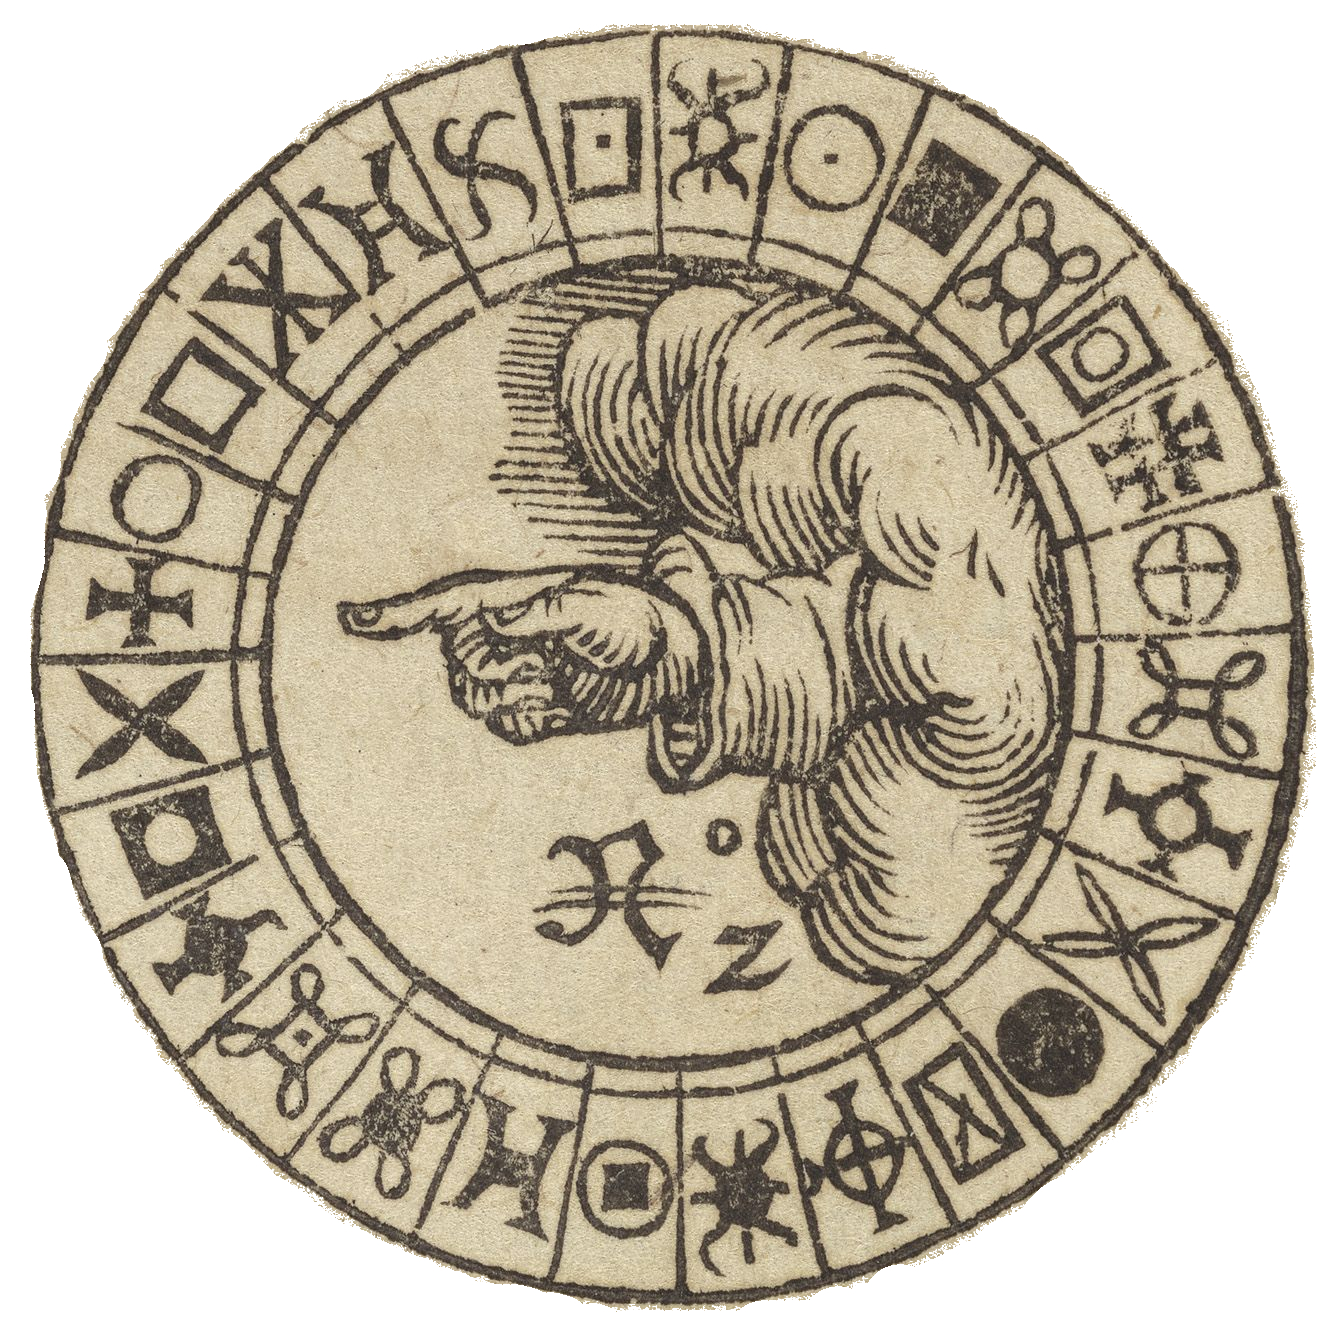
\includegraphics[width=4cm]{../resources/jpg/2.3.functions/symbol2.jpg}
\end{figure}
\pagebreak


% ============================== 0078 Theorem 2346 ================================
\subsection[The ceiling of a real number and an integer.]
    {
        \color{section}Theorem 78. \color{black} The ceiling of a real and an integer.
    }
\documentclass[preview]{standalone}
\usepackage{amssymb, amsthm}
\usepackage{mathtools}
\usepackage{bm}


\newtheorem{theorem}{Theorem}
\renewcommand\qedsymbol{$\blacksquare$}


\begin{document}


\begin{theorem}[\textbf{2346}]
    Let \bm{$\lambda$} be a real number, 
    and let \bm{$\zeta$} be an integer. 
    \begin{equation*}
        \bm{\lceil \lambda + \zeta \rceil 
            =
        \lceil \lambda \rceil + \zeta}
    \end{equation*}
\end{theorem}

\begin{proof}
    Given \bm{$\lceil \lambda \rceil$}, by the properties for ceiling functions we have
    \begin{equation*}
        \Big \langle \lceil \lambda \rceil - 1 \Big \rangle
            < 
        \Big \langle \lambda \Big \rangle
            \le 
        \Big \langle \lceil \lambda \rceil \Big \rangle
    \end{equation*}
    By the additive compatibility law from the order axioms, that is
    \begin{equation*}
        \Big \langle \big[ \lceil \lambda \rceil + \zeta \big] - 1 \Big \rangle
            < 
        \Big \langle \lambda + \zeta \Big \rangle
            \le 
        \Big \langle \lceil \lambda \rceil + \zeta \Big \rangle
    \end{equation*} 
    $\therefore \text{\space} \bm{
    \lceil \lambda + \zeta \rceil = \lceil \lambda \rceil + \zeta$},
    by the properties for ceiling functions.
    
\end{proof}


\end{document}
\sep


% ============================== 0079 Theorem 2347a ===============================
\subsection[If a floor is less than an integer.]
    {
        \color{section}Theorem 79. \color{black} If a floor is less than an integer.
    }
\documentclass[preview]{standalone}
\usepackage{amssymb, amsthm}
\usepackage{mathtools}
\usepackage{bm}


\newtheorem{theorem}{Theorem}
\renewcommand\qedsymbol{$\blacksquare$}


\begin{document}


\begin{theorem}[\textbf{2347a}]
    Let \bm{$\lambda$} be a real number, 
    and let \bm{$\zeta$} be an integer. 
    \begin{equation*}
        \bm{\big \langle \lambda < \zeta \big \rangle
            \textbf{ if and only if } 
        \big \langle \lfloor \lambda \rfloor < \zeta \big \rangle
        }
    \end{equation*}
\end{theorem}

\begin{proof}
    Assume \bm{$\lambda < \zeta$}. 
    By the properties of the floor function,
    \bm{$\lfloor \lambda \rfloor \leq \lambda$}. 
    Thus,
    \begin{equation*}
        \Big \langle \lfloor \lambda \rfloor \Big \rangle
            \leq 
        \Big \langle \lambda \Big \rangle
            < 
        \Big \langle \zeta \Big \rangle
    \end{equation*}
    It immediately follows from transitivity that 
    \bm{$\lfloor \lambda \rfloor < \zeta$}.
    \\ \\
    In the converse case, 
    assume \bm{$\lfloor \lambda \rfloor < \zeta$}. 
    Since \bm{$\lfloor \lambda \rfloor$} and \bm{$\zeta$} are integers, 
    we can infer from additive compatibility that
    \bm{$\lfloor \lambda \rfloor + 1 \le \zeta$}. 
    And by the properties of the floor function, we have
    \begin{equation*}
        \Big \langle \lfloor \lambda \rfloor \Big \rangle
            \leq 
        \Big \langle \lambda \Big \rangle 
            <
        \Big \langle \lfloor \lambda \rfloor + 1 \Big \rangle
    \end{equation*}
    Thus,
    \begin{equation*}
        \Big \langle \lfloor \lambda \rfloor \Big \rangle
            \le 
        \Big \langle \lambda \Big \rangle
            < 
        \Big \langle \lfloor \lambda \rfloor + 1 \Big \rangle
            \le 
        \Big \langle \zeta \Big \rangle
    \end{equation*}
    This statement says that \bm{$\lambda < \zeta$}.
    \\ \\
    $\therefore \text{\space} \bm{
        \big \langle \lambda < \zeta \big \rangle
            \textbf{ \emph{if and only if} } 
        \big \langle \lfloor \lambda \rfloor < \zeta \big \rangle
    }$.
\end{proof}


\end{document}
\pagebreak


% ============================== 0080 Theorem 2347b ===============================
\subsection[If an interger is less than a ceiling.]
    {
        \color{section}Theorem 80. \color{black} If an interger is less than a ceiling.
    }
\documentclass[preview]{standalone}
\usepackage{amssymb, amsthm}
\usepackage{mathtools}
\usepackage{bm}


\newtheorem{theorem}{Theorem}
\renewcommand\qedsymbol{$\blacksquare$}


\begin{document}


\begin{theorem}[\textbf{2347b}]
    Let \bm{$\lambda$} be a real number, 
    and let \bm{$\zeta$} be an integer. 
    \begin{equation*}
        \bm{
            \big \langle \zeta < \lambda \big \rangle
                \textbf{ if and only if } 
            \big \langle \zeta < \lceil \lambda \rceil \big \rangle
        }
    \end{equation*}
\end{theorem}

\begin{proof}
    Assume \bm{$\zeta < \lambda$}.
    By the properties of the ceiling function, 
    \bm{$\lambda \leq \lceil \lambda \rceil$}.
    Thus,
    \begin{equation*}
        \Big \langle \zeta \Big \rangle
            <
        \Big \langle \lambda \Big \rangle
            \leq
        \Big \langle \lceil \lambda \rceil \Big \rangle
    \end{equation*}
    It immediately follows that
    \bm{$\zeta < \lceil \lambda \rceil$}.
    \\ \\
    In the converse case, assume
    \bm{$\zeta < \lceil \lambda \rceil$}.
    Since \bm{$\lceil \lambda \rceil$} and \bm{$\zeta$} are integers,
    by the additive compatibility law from the order axioms, we can infer 
    \bm{$\zeta \leq \lceil \lambda \rceil - 1$}.
    And by the properties of the ceiling function, we have
    \begin{equation*}
        \Big \langle \lceil \lambda \rceil - 1 \Big \rangle
            <
        \Big \langle \lambda \Big \rangle
            \leq
        \Big \langle \lceil \lambda \rceil \Big \rangle
    \end{equation*}
    Thus,
    \begin{equation*}
        \Big \langle \zeta \Big \rangle
            \leq
        \Big \langle \lceil \lambda \rceil - 1 \Big \rangle
            <
        \Big \langle \lambda \Big \rangle
            \leq
        \Big \langle \lceil \lambda \rceil \Big \rangle
    \end{equation*}
    This statement says that \bm{$\zeta < \lambda$}.
    \\ \\
    $\therefore \text{\space} \bm{
        \big \langle \zeta < \lambda \big \rangle
            \textbf{ \emph{if and only if} } 
        \big \langle \zeta < \lceil \lambda \rceil \big \rangle
    $}.
\end{proof}


\end{document}
\sep


% ============================== 0081 Theorem 2348a ===============================
\subsection[If a ceiling is less than or equal to...]
    {
        \color{section}Theorem 81. \color{black} If a ceiling is less than or equal to...
    }
\documentclass[preview]{standalone}
\usepackage{amssymb, amsthm}
\usepackage{mathtools}
\usepackage{bm}


\newtheorem{theorem}{Theorem}
\renewcommand\qedsymbol{$\blacksquare$}


\begin{document}


\begin{theorem}[\textbf{2348a}]
    Let \bm{$\lambda$} be a real number, 
    and let \bm{$\zeta$} be an integer.
    \begin{equation*}
        \bm{
        \big \langle \lambda \le \zeta \big \rangle
            \textbf{ if and only if } 
        \big \langle \lceil \lambda \rceil \le \zeta \big \rangle
        }
    \end{equation*}
\end{theorem}

\begin{proof}
    Direct form by the contrapositive. 
    Assume the negation of the direct consequent,
    such that \bm{$\lceil \lambda \rceil > \zeta$}. 
    By Theorem 80, 
    \bm{$\lambda > \zeta$}.
    Thus,
    \begin{equation*}
        \bigg[
            \Big \langle \lambda \Big \rangle
                \leq 
            \Big \langle \zeta \Big \rangle
        \bigg]
            \rightarrow 
        \bigg[
            \Big \langle \lceil \lambda \rceil \Big \rangle
                \leq 
            \Big \langle \zeta \Big \rangle
        \bigg]
    \end{equation*}
    Converse form by the contrapositive. 
    Assume the negation of the direct hypothesis, 
    such that \bm{$\lambda > \zeta$}.
    By Theorem 80, \bm{$\lceil \lambda \rceil > \zeta$}. 
    Thus,
    \begin{equation*}
        \bigg[
            \Big \langle \lceil \lambda \rceil \Big \rangle
                \leq 
            \Big \langle \zeta \Big \rangle
        \bigg]
            \rightarrow 
        \bigg[
            \Big \langle \lambda \Big \rangle
                \leq 
            \Big \langle \zeta \Big \rangle
        \bigg]
    \end{equation*}
    $\therefore \text{\space} \bm{
        \big \langle \lambda \le \zeta \big \rangle
            \textbf{ \emph{if and only if} } 
        \big \langle \lceil \lambda \rceil \le \zeta \big \rangle}
    $.
\end{proof}


\end{document}
\pagebreak


% ============================== 0082 Theorem 2348b ===============================
\begin{figure}[!h]
    \centering
    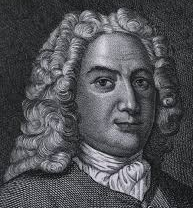
\includegraphics[width=11cm]{../resources/jpg/2.3.functions/bernoulli.jpg}
    \caption*{Johann Bernoulli.}
\end{figure}
\subsection[If an integer is less than or equal to...]
    {
        \color{section}Theorem 82. \color{black} If an integer is less than or equal to...
    }
\documentclass[preview]{standalone}
\usepackage{amssymb, amsthm}
\usepackage{mathtools}
\usepackage{bm}


\newtheorem{theorem}{Theorem}
\renewcommand\qedsymbol{$\blacksquare$}


\begin{document}


\begin{theorem}[\textbf{2348b}]
    Let \bm{$\lambda$} be a real number, 
    and let \bm{$\zeta$} be an integer. 
    \begin{equation*}
        \bm{
        \big \langle \zeta \le \lambda \big \rangle
            \textbf{ if and only if }
        \big \langle \zeta \le \lfloor \lambda \rfloor \big \rangle}
    \end{equation*}
\end{theorem}

\begin{proof}
    Direct form by the contrapositive.
    Assume the negation of the direct consequent,
    such that \bm{$\zeta > \lfloor \lambda \rfloor$}.
    By Theorem 79, \bm{$\zeta > \lambda$}.
    Thus,
    \begin{equation*}
        \bigg[
            \Big \langle \zeta \Big \rangle
                \leq 
            \Big \langle \lambda \Big \rangle
        \bigg]
            \rightarrow 
        \bigg[
            \Big \langle \zeta \Big \rangle
                \leq 
            \Big \langle \lfloor \lambda \rfloor \Big \rangle
        \bigg]
    \end{equation*}
    Converse form by the contrapositive.
    Assume the negation of the direct hypothesis,
    such that \bm{$\zeta > \lambda$}.
    By Theorem 79, 
    \bm{$\zeta > \lfloor \lambda \rfloor$}.
    Thus,
    \begin{equation*}
        \bigg[
            \Big \langle \zeta \Big \rangle
                \leq 
            \Big \langle \lfloor \lambda \rfloor \Big \rangle
        \bigg]
            \rightarrow 
        \bigg[
            \Big \langle \zeta \Big \rangle
                \leq 
            \Big \langle \lambda \Big \rangle
        \bigg]
    \end{equation*}
    $\therefore \text{\space} \bm{
        \big \langle \zeta \le \lambda \big \rangle
            \textbf{ \emph{if and only if} }
        \big \langle \zeta \le \lfloor \lambda \rfloor \big \rangle}
    $.
\end{proof}


\end{document}
\pagebreak


% ============================== 0083 Theorem 2349 ================================
\subsection[Parity for flooring a half.]
    {
        \color{section}Theorem 83. \color{black} Parity for flooring a half.
    }
\documentclass[preview]{standalone}
\usepackage{amssymb, amsthm}
\usepackage{mathtools}
\usepackage{bm}


\newtheorem{theorem}{Theorem}
\renewcommand\qedsymbol{$\blacksquare$}


\begin{document}


\begin{theorem}[\textbf{2349}]
    Let \bm{$\zeta$} be an integer. 
    \begin{equation*}
        \textbf{If } \bm{\zeta} \textbf{ is even, then } 
        \bm{
            \bigg \lfloor \frac{\zeta}{2} \bigg \rfloor
                = 
            \frac{\zeta}{2}
        }
        \textbf{; if } \bm{\zeta} \textbf{ is odd, then } 
        \bm{
            \bigg \lfloor \frac{\zeta}{2} \bigg \rfloor 
                = 
            \frac{ \big \langle \zeta - 1 \big \rangle }{2}
        }
    \end{equation*}
\end{theorem}

\begin{proof}
    By cases. 
    \\ \\
    \bm{$(i)$} Assume \bm{$\zeta$} is even.
    By the definition for even numbers,
    there exists an integer \bm{$\iota$} such that 
    \bm{$\zeta = 2 \iota$}. 
    Thus, by that identity for \bm{$\zeta$}, 
    and by the multiplicative inverse from the field axioms,
    \begin{equation*}
        \bigg( \frac{\zeta}{2} \bigg)
            = 
        \bigg( \frac{2 \iota}{2} \bigg)
            = 
        \Big \langle \iota \Big \rangle
    \end{equation*}
    By that identity \bm{$\iota$}, 
    and by the definition for the floor function,
    \begin{equation*}
        \Big \lfloor \frac{\zeta}{2} \Big \rfloor
            =
        \Big \lfloor \iota \Big \rfloor 
            = 
        \Big \langle \iota \Big \rangle
    \end{equation*}
    $\therefore \textbf{if } \bm{\zeta} \textbf{ is even, then } 
        \bm{
            \Big \lfloor \frac{\zeta}{2} \Big \rfloor
                = 
            \frac{\zeta}{2}
    }$, 
    by the identity \bm{$\iota$}.
    \\ \\
    \bm{$(ii)$} Assume \bm{$\zeta$} is odd. 
    By the definition for odd numbers,
    there exists an integer \bm{$\iota$} such that 
    \bm{$\zeta = 2 \iota + 1$}.
    Thus, by that identity for \bm{$\zeta$}, 
    by the multiplicative inverse from the field axioms,
    and by the definition for floor functions,
    \begin{equation*}
        \bigg \lfloor 
            \frac{\zeta}{2}
        \bigg \rfloor 
            = 
        \bigg \lfloor 
            \frac{2 \iota + 1}{2}
        \bigg \rfloor 
            = 
        \bigg \lfloor
            \iota + \frac{1}{2}
        \bigg \rfloor 
            = 
        \Big \langle \iota \Big \rangle
    \end{equation*}
    Also, by that identity for \bm{$\zeta$},
    and by the additive and multiplicative inverse from the field axioms,
    \begin{equation*}
        \Bigg( \frac{\big \langle \zeta - 1 \big \rangle }{2} \Bigg)
            = 
        \Bigg( \frac{\big[ \big \langle 2 \iota + 1 \big \rangle - 1 \big]}{2} \Bigg)
            = 
        \Bigg( \frac{2 \iota}{2} \Bigg)
            = 
        \Big \langle \iota \Big \rangle
    \end{equation*} 
    $\therefore \textbf{if } \bm{\zeta} \textbf{ is odd, then } 
    \bm{
        \Big \lfloor \frac{\zeta}{2} \Big \rfloor 
            = 
        \frac{ \langle \zeta - 1 \rangle }{2}
    }$, 
    by the identity \bm{$\iota$}.
\end{proof}


\end{document}
\begin{figure}[!h]
    \centering
    
\includegraphics[width=2.5cm]{../resources/jpg/2.3.functions/symbol3.png}
\end{figure}
\pagebreak


% ============================== 0084 Theorem 2350 ================================
\subsection[The ceiling and floor of negative numbers.]
    {
        \color{section}Theorem 84. \color{black} The ceiling and floor of negatives.
    }
\documentclass[preview]{standalone}
\usepackage{amssymb, amsthm}
\usepackage{mathtools}
\usepackage{bm}


\newtheorem{theorem}{Theorem}
\renewcommand\qedsymbol{$\blacksquare$}


\begin{document}


\begin{theorem}[\textbf{2350}]
    Let \bm{$\zeta$} be a real number. 
    \begin{equation*}
        \bm{
            \lfloor - \zeta \rfloor 
                = 
            - \lceil \zeta \rceil
                \textbf{, and }
            \lceil - \zeta \rceil
                = 
            - \lfloor \zeta \rfloor
        }.
    \end{equation*}
\end{theorem}


\begin{proof}
    By cases.
    \\ \\
    \bm{$(i)$} By the multiplicative compatibility laws from the order axioms,
    and by the properties for ceiling functions,
    there exists an integer \bm{$\lceil \zeta \rceil = \lambda$} such that
    \begin{equation*}
        \Bigg\{
            \Big \langle \lambda - 1 \Big \rangle
                <
            \Big \langle \zeta \Big \rangle
                \leq
            \Big \langle \lambda \Big \rangle
        \Bigg\}
            \equiv
        \Bigg\{
            \Big \langle - \lambda + 1 \Big \rangle 
                > 
            \Big \langle - \zeta \Big \rangle
                \ge 
            \Big \langle - \lambda \Big \rangle
        \Bigg\}
    \end{equation*}
    By the properties for floor functions, 
    \bm{$\lfloor - \zeta \rfloor = - \lambda$}.
    And \bm{$-1 \times \lceil \zeta \rceil = - \lambda$}, 
    by the multiplicative equality property for equations.
    Thus, \bm{$\lfloor - \zeta \rfloor = - \lceil \zeta \rceil$}, 
    by the identity \bm{$- \lambda$}.
    \\ \\
    \bm{$(ii)$} By the multiplicative compatibility laws from the order axioms,
    and by the properties of floor functions,
    there exists an integer \bm{$\lfloor \zeta \rfloor = \lambda$} such that
    \begin{equation*}
        \Bigg\{
            \Big \langle \lambda \Big \rangle
                \le 
            \Big \langle \zeta \Big \rangle
                < 
            \Big \langle \lambda + 1 \Big \rangle
        \Bigg\}
            \equiv
        \Bigg\{
            \Big \langle - \lambda \Big \rangle
                \ge 
            \Big \langle - \zeta \Big \rangle
                > 
            \Big \langle - \lambda - 1 \Big \rangle
        \Bigg\}
    \end{equation*}
    By the properties of ceiling functions,
    \bm{$\lceil - \zeta \rceil = - \lambda$}. 
    And  
    \bm{$- 1 \times \lfloor \zeta \rfloor = - \lambda$}, 
    by the multiplicative property for equations.
    Thus,
    \bm{$\lceil - \zeta \rceil = - \lfloor \zeta \rfloor$},
    by the identity \bm{$- \lambda$}.
    \\ \\
    $\therefore \text{\space}
    \bm{
            \lfloor - \zeta \rfloor 
                = 
            - \lceil \zeta \rceil
                \textbf{, and }
            \lceil - \zeta \rceil
                = 
            - \lfloor \zeta \rfloor
    }$.
\end{proof}


\end{document}
%\sep
\vspace{2\baselineskip}
\begin{figure}[!h]
    \centering
    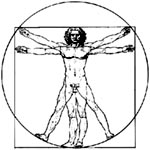
\includegraphics[width=4cm]{../resources/jpg/2.3.functions/symbol4.jpg}
\end{figure}
\pagebreak


% ============================== 0085 Theorem 2366 ================================
\begin{figure}[!h]
    \centering
    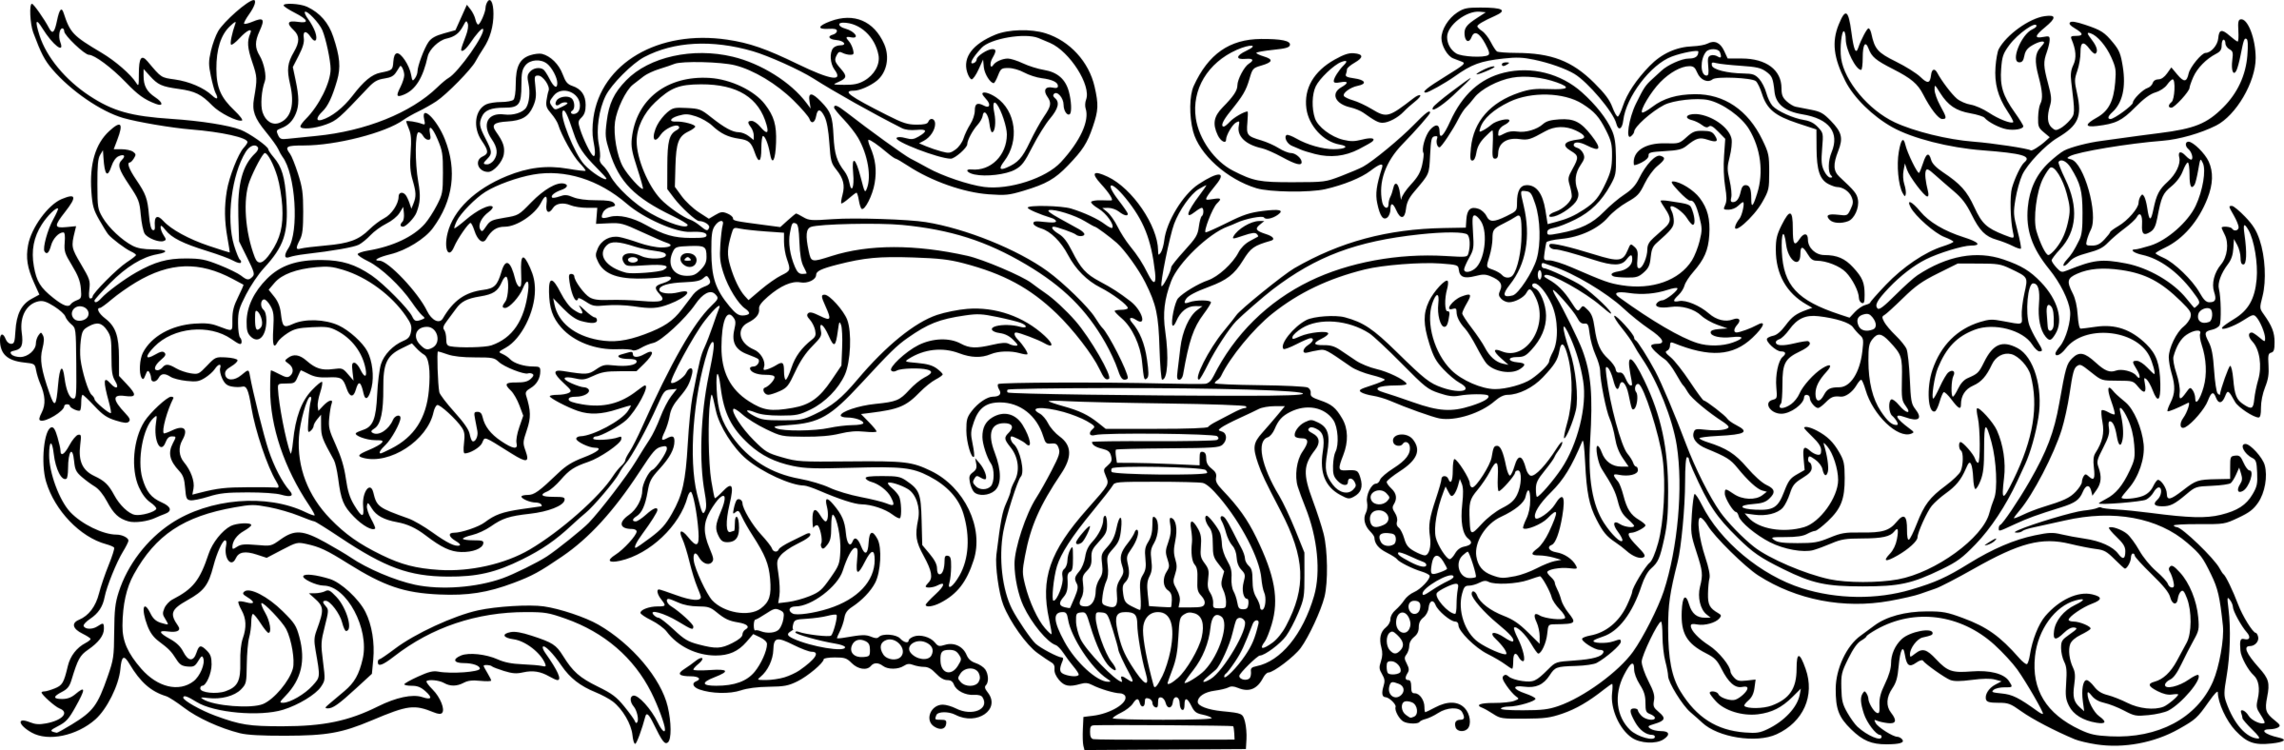
\includegraphics[width=14cm]{../resources/jpg/2.3.functions/border1.png}
\end{figure}
\subsection[The inverse of compositions.]
    {
        \color{section}Theorem 85. \color{black} The inverse of compositions.
    }
\documentclass[preview]{standalone}
\usepackage{amssymb, amsthm}
\usepackage{mathtools}
\usepackage{bm}


\newtheorem{theorem}{Theorem}
\renewcommand\qedsymbol{$\blacksquare$}


\begin{document}


\begin{theorem}[\textbf{2366}]
    Let \bm{$\sigma$} be the invertible function 
    \bm{$\sigma : \Theta \rightarrow \Omega$}, 
    and let \bm{$\phi$} be the invertible function 
    \raggedright \bm{$\phi : \Phi \rightarrow \Theta$}. 
    \begin{equation*}
        \text{The inverse of the composition }
        \bm{\sigma \circ \phi}
        \text{ is given by }
    \end{equation*}
    \begin{equation*}
        \bm{
            \big \langle \sigma \circ \phi \big \rangle ^{-1} 
                = \phi ^{-1} \circ \sigma ^{-1}
            }
    \end{equation*}
\end{theorem}

\begin{proof}
    By Theorem 66 and Theorem 67, and by the definition for bijective functions, 
    \bm{$\sigma \circ \phi$} is invertible. 
    Thus, 
    \begin{equation*}
        \big \langle \sigma \circ \phi \big \rangle ^{-1} 
            \circ 
        \big \langle \sigma \circ \phi \big \rangle 
            = 
        \iota_{\alpha}
    \end{equation*}
    What remains to be determined is whether 
    \bm{$
        \big \langle \phi ^{-1} \circ \sigma ^{-1} \big \rangle
            \circ 
        \big \langle \sigma \circ \phi \big \rangle
            = 
        \iota_{\alpha}$
    }. 
    Let \bm{$\alpha$} be an element in the domain \bm{$\Phi$} such that 
    \begin{equation*}
        \big[
            \big \langle \phi ^{-1} \circ \sigma ^{-1} \big \rangle 
                \circ 
            \big \langle \sigma \circ \phi \big \rangle
        \big] 
            \big[ \alpha \big] 
            = 
        \alpha
    \end{equation*}
    By the definition for the composition of functions, 
    that is 
    \begin{equation*}
        \phi ^{-1} \text{\space} \big[ 
            \sigma ^{-1} \text{\space} \big[ 
                \sigma \text{\space} \big[ 
                    \phi \text{\space} \big[
                        \alpha \text{\space}
                    \big]
                \big]
            \big]
        \big]
             = 
        \alpha
    \end{equation*}
    Clearly, 
    \bm{$
        \big \langle \phi ^{-1} \circ \sigma ^{-1} \big \rangle
            \circ 
        \big \langle \sigma \circ \phi \big \rangle
            = 
        \iota_{\alpha}$}
    \\ \\
    $\therefore \text{ \emph{the inverse of the composition} } \bm{
        \sigma \circ \phi 
        \text{ \emph{is given by} }
        \big \langle \sigma \circ \phi \big \rangle ^{-1} 
            = 
        \phi^{-1} \circ \sigma^{-1}
    }$.
\end{proof}


\end{document}
\begin{figure}[!h]
    \centering
    
\includegraphics[width=3cm]{../resources/jpg/2.3.functions/symbol6.jpg}
\end{figure}
\pagebreak


% ============================== 0086 Theorem 2367a ===============================
\subsection[Characteristic functions on intersections.]
    {
        \color{section}Theorem 86. \color{black} Characteristic functions on intersection.
    }
\documentclass[preview]{standalone}
\usepackage{amssymb, amsthm}
\usepackage{mathtools}
\usepackage{bm}


\newtheorem{theorem}{Theorem}
\renewcommand\qedsymbol{$\blacksquare$}


\begin{document}


\begin{theorem}[\textbf{2367a}]
    Suppose that \bm{$\mathrm{A}$}, and \bm{$\Lambda$} are sets with universal set \bm{$\Omega$}. 
    \begin{center}
    Let \bm{$\lambda_{\mathrm{A} \cap \Lambda}$} be the characteristic function 
    \bm{$\lambda_{\mathrm{A} \cap \Lambda}: \Omega \rightarrow \{0, 1\}$}, 
    let \bm{$\lambda_{\mathrm{A}}$} be the characteristic function 
    \bm{$\lambda_{\mathrm{A}}: \Omega \rightarrow \{0, 1\}$},
    and let \bm{$\lambda_{\Lambda}$} be the characteristic function  
    \bm{$\lambda_{\Lambda}: \Omega \rightarrow \{0, 1\}$}.
    \end{center}
    \vspace{1\baselineskip}
    \begin{equation*}
        \bm{
            \lambda_{\mathrm{A} \cap \Lambda}\big[ \iota \big] 
                = 
            \lambda_{\mathrm{A}}\big[ \iota \big] 
                \times 
            \lambda_{\Lambda}\big[ \iota \big]
            }
    \end{equation*}
\end{theorem}

\begin{proof}
    By cases. There are two cases under consideration. 
    $(i)$ \bm{$\iota$} is a member of \bm{$\mathrm{A} \cap \Lambda$}, or 
    $(ii)$ it is not the case that \bm{$\iota$} is a member of \bm{$\mathrm{A} \cap \Lambda$}.
    \\ \\
    \bm{$(i)$} Suppose \bm{$\iota$} were an element in \bm{$\mathrm{A} \cap \Lambda$}.
    Note that, 
    \bm{$\lambda_{\mathrm{A} \cap \Lambda}\big[ \iota \big] = 1$},
    by the definition for characteristic functions.
    Now, by the definition for the intersection of sets, 
    and by the definition for characteristic functions,
    \begin{equation*}
        \bigg[
            \Big \langle \iota \in \mathrm{A} \Big \rangle 
                \land 
            \Big \langle \iota \in \Lambda \Big \rangle
        \bigg]
            \equiv
        \bigg[
            \Big \langle \lambda_\mathrm{A} \big[ \iota \big] = 1 \Big \rangle
                \land
            \Big \langle \lambda_{\Lambda} \big[ \iota \big] = 1 \Big \rangle
        \bigg]
    \end{equation*}
    It follows immediately from logical identity, 
    and by multiplicative identity 
    from the field axioms that 
    \bm{$
        \lambda_{\mathrm{A} \cap \Lambda} \big[ \iota \big] 
            = 
        \lambda_{\mathrm{A}} \big[ \iota \big] 
            \times 
        \lambda_{\Lambda} \big[ \iota \big]
    $}, in this case.
    \\ \\
    \bm{$(ii)$} Suppose it were not the case that \bm{$\iota$} were an element in 
    \bm{$\mathrm{A} \cap \Lambda$}.
    Note that, \bm{$\lambda_{\mathrm{A} \cap \Lambda} \big[ \iota \big] = 0$},
    by the definition for characteristic functions.
    Now. by the definitions for set intersection and set membership, 
    and by DeMorgans law for set intersection,
    \begin{equation*}
        \bigg[
            \iota \notin \Big \langle 
                \mathrm{A} \cap \Lambda 
            \Big \rangle
        \bigg]
            \equiv
        \lnot \bigg[
            \Big \langle \iota \in \mathrm{A} \Big \rangle
                \land
            \Big \langle \iota \in \Lambda \Big \rangle
        \bigg]
            \equiv
        \bigg[
            \Big \langle \iota \notin \mathrm{A} \Big \rangle
                \lor
            \Big \langle \iota \notin \Lambda \Big \rangle
        \bigg]
    \end{equation*}
    And, by the definition for characteristic functions,
    \begin{equation*}
        \bigg[
            \Big \langle \iota \notin \mathrm{A} \Big \rangle
                \lor
            \Big \langle \iota \notin \Lambda \Big \rangle
        \bigg]
            \equiv
        \bigg[
            \Big \langle \lambda_{\mathrm{A}} \big[ \iota \big] = 0 \Big \rangle 
                \lor 
            \Big \langle \lambda_{\Lambda} \big[ \iota \big] = 0 \Big \rangle
        \bigg]
    \end{equation*}
    Without loss of generality we can suppose 
    \bm{$\lambda_{\mathrm{A}} \big[ \iota \big] = 0$}. 
    It follows immediately from logical identity, 
    and from the multiplicative property for zero that 
    \bm{$\lambda_{\mathrm{A} \cap \Lambda} \big[ \iota \big] 
        = 
     0 \times \lambda_{\mathrm{A}} \big[ \iota \big] = 0$}. 
    Thus, 
    \bm{$\lambda_{\mathrm{A} \cap \Lambda} \big[ \iota \big] 
        = 
    \lambda_{\mathrm{A}} \big[ \iota \big] 
        \times 
    \lambda_{\Lambda} \big[ \iota \big]$}, in this case.
\end{proof}


\end{document}
\begin{figure}[!h]
    \centering
    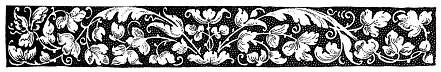
\includegraphics[width=14.25cm]{../resources/jpg/2.3.functions/border2.jpg}
\end{figure}
\pagebreak


% ============================== 0087 Theorem 2367b ===============================
\subsection[Characteristic functions on unions.]
    {
        \color{section}Theorem 87. \color{black} Characteristic functions on unions.
    }
\documentclass[preview]{standalone}
\usepackage{amssymb, amsthm}
\usepackage{mathtools}
\usepackage{bm}


\newtheorem{theorem}{Theorem}
\renewcommand\qedsymbol{$\blacksquare$}


\begin{document}


\begin{theorem}[\textbf{2367b}]
    Suppose that \bm{$\mathrm{A}$}, and \bm{$\Lambda$} are sets with universal set \bm{$\Omega$}.
    \begin{center}
        Let \bm{$\lambda_{\mathrm{A} \cup \Lambda}$} be the characteristic function 
        \bm{$\lambda_{\mathrm{A} \cup \Lambda} : \Omega \rightarrow \{0, 1\}$},
        let \bm{$\lambda_{\mathrm{A}}$} be the characteristic function 
        \bm{$\lambda_{\mathrm{A}} : \Omega \rightarrow \{0, 1\}$},
        and let \bm{$\lambda_{\Lambda}$} be the characteristic function 
        \bm{$\lambda_{\Lambda}: \Omega \rightarrow \{0, 1\}$}.
    \end{center}
    \begin{equation*}
        \bm{
            \lambda_{\mathrm{A} \cup \Lambda} \big[ \iota \big] 
                = 
            \lambda_{\mathrm{A}} \big[ \iota \big] 
                + 
            \lambda_{\Lambda} \big[ \iota \big] 
                - 
            \lambda_{\mathrm{A}} \big[ \iota \big]
                \times 
            \lambda_{\Lambda} \big[ \iota \big]
        }
    \end{equation*}
\end{theorem}

\begin{proof}
    By cases. There are two major cases under consideration.
    \\ \\
    \bm{$(i)$} Assume \bm{$\iota$} is not an element in \bm{$\mathrm{A} \cup \Lambda$}. 
    Note that, by the definition for characteristic functions, 
    \bm{$\lambda_{\mathrm{A} \cup \Lambda}\big[ \iota \big] = 0$}.
    Now, by the definition for set union 
    \bm{$\iota$} is in neither \bm{$\mathrm{A}$} nor \bm{$\Lambda$}.
    So \bm{$\lambda_{\mathrm{A}} \big[ \iota \big] = 0$}, 
    and \bm{$\lambda_{\Lambda} \big[ \iota \big] = 0$}. 
    Hence,
    \begin{equation*}
        \bigg \langle
            \lambda_{\mathrm{A}} \big[ \iota \big] 
                + 
            \lambda_{\Lambda} \big[ \iota \big] 
                - 
            \lambda_{\mathrm{A}} \big[ \iota \big] 
                \times 
            \lambda_{\Lambda} \big[ \iota \big] 
        \bigg \rangle
            =
        \bigg \langle 
            0 + 0 - 0 \times 0 
        \bigg \rangle
            =
        \bigg \langle 
            0
        \bigg \rangle
    \end{equation*}
    $\therefore \text{\space} \bm{
        \lambda_{\mathrm{A} \cup \Lambda} \big[ \iota \big] 
            = 
        \lambda_{\mathrm{A}} \big[ \iota \big] 
            + 
        \lambda_{\Lambda} \big[ \iota \big] 
            - 
        \lambda_{\mathrm{A}} \big[ \iota \big]
            \times 
        \lambda_{\Lambda} \big[ \iota \big]
    }$.
    \\ \\
    \bm{$(ii)$} Assume \bm{$\iota$} is an element in \bm{$\mathrm{A} \cup \Lambda$}. 
    By the definition for characteristic functions 
    \bm{$\lambda_{\mathrm{A} \cup \Lambda} \big[ \iota \big] = 1$}. 
    Also, by the definition for set union 
    \begin{equation*}        
        \Big \langle \iota \in \mathrm{A} \Big \rangle 
            \lor 
        \Big \langle \iota \in \Lambda \Big \rangle
    \end{equation*}
    There are three subcases. 
    \\ \\
    \bm{$(a)$} Suppose \bm{$\iota$} is an element in \bm{$\mathrm{A}$}, but not in \bm{$\Lambda$}.
    By the definition for characteristic functions 
    \bm{$\lambda_{\mathrm{A}} \big[ \iota \big] = 1$}, 
    and \bm{$\lambda_{\Lambda} \big[ \iota \big] = 0$}. 
    Thus,
    \begin{equation*}
        \bigg \langle
            \lambda_{\mathrm{A}} \big[ \iota \big] 
                + 
            \lambda_{\Lambda} \big[ \iota \big] 
                - 
            \lambda_{\mathrm{A}} \big[ \iota \big] 
                \times 
            \lambda_{\Lambda} \big[ \iota \big] 
        \bigg \rangle
            =
        \bigg \langle 
            1 + 0 - 1 \times 0 
        \bigg \rangle
            =
        \bigg \langle 
            1
        \bigg \rangle
    \end{equation*} 
    \bm{$(b)$} Suppose \bm{$\iota$} is not an element in \bm{$\mathrm{A}$}, 
    but is an element in \bm{$\Lambda$}. 
    Without loss of generality this case has the same result as case $(a)$.
    \\ \\
    \bm{$(c)$} Suppose \bm{$\iota$} is in the intersection of \bm{$\mathrm{A}$} and \bm{$\Lambda$}.
    \begin{equation*}
        \bigg \langle
            \lambda_{\mathrm{A}} \big[ \iota \big] 
                + 
            \lambda_{\Lambda} \big[ \iota \big] 
                - 
            \lambda_{\mathrm{A}} \big[ \iota \big] 
                \times 
            \lambda_{\Lambda} \big[ \iota \big] 
        \bigg \rangle
            =
        \bigg \langle 
            1 + 1 - 1 \times 1 
        \bigg \rangle
            =
        \bigg \langle 
            1
        \bigg \rangle
    \end{equation*}
    $\therefore \text{\space} \bm{
        \lambda_{\mathrm{A} \cup \Lambda} \big[ \iota \big] 
            = 
        \lambda_{\mathrm{A}} \big[ \iota \big] 
            + 
        \lambda_{\Lambda} \big[ \iota \big] 
            - 
        \lambda_{\mathrm{A}} \big[ \iota \big]
            \times 
        \lambda_{\Lambda} \big[ \iota \big]
    }$.
\end{proof}


\end{document}
\pagebreak


% ============================== 0088 Theorem 2367c ===============================
\subsection[Characteristic functions on a complement.]
    {
        \color{section}Theorem 88. \color{black} Characteristic functions on complements
    }
\documentclass[preview]{standalone}
\usepackage{amssymb, amsthm}
\usepackage{mathtools}
\usepackage{bm}


\newtheorem{theorem}{Theorem}
\renewcommand\qedsymbol{$\blacksquare$}


\begin{document}


\begin{theorem}[\textbf{2367c}]
    Let \bm{$\Lambda$} be a set with universal set \bm{$\Omega$}. 
    Let \bm{$\lambda_{\overline{\Lambda}}$} be the characteristic function 
    \bm{$\lambda_{\overline{\Lambda}}: \Omega \rightarrow \{0, 1\}$}. 
    \begin{equation*}
        \bm{
            \lambda_{\overline{\Lambda}} \big[ \iota \big] 
                = 
            1 - \lambda_{\Lambda} \big[ \iota \big]
        }
    \end{equation*}
\end{theorem}

\begin{proof}
    By cases. There are two cases. 
    Either $(i)$ \bm{$\iota$} is in \bm{$\Lambda$},
    xor $(ii)$ \bm{$\iota$} is in \bm{$\overline{\Lambda}$}.
    \\ \\
    \bm{$(i)$} Let \bm{$\iota$} be an element in \bm{$\Lambda$}. 
    By the double negation law, 
    by the definition for set membership,
    by the definition for set complement,
    and again by the defintion for set membership, that is
    \begin{equation*}
        \lnot \bigg[ \lnot \Big \langle \iota \in \Lambda \Big \rangle \bigg]
            \equiv
        \lnot \Big \langle \iota \notin \Lambda \Big \rangle
            \equiv
        \lnot \Big \langle \iota \in \overline{\Lambda} \Big \rangle
            \equiv
        \Big \langle \iota \notin \overline{\Lambda} \Big \rangle
    \end{equation*}
    Thus, by the definition for characteristic functions 
    \begin{equation*}
        \Big \langle 
            \lambda_{\overline{\Lambda}} \big[ \iota \big] = 0
        \Big \rangle
            \land
        \Big \langle 
            \lambda_{\Lambda} \big[ \iota \big] = 1
        \Big \rangle
    \end{equation*}
    $\therefore \text{\space} \bm{
        \lambda_{\overline{\Lambda}} \big[ \iota \big] 
            = 
        1 - \lambda_{\Lambda} \big[ \iota \big]
    }$.
    \\ \\
    \bm{$(ii)$} Let \bm{$\iota$} be an element in \bm{$\overline{\Lambda}}$.
    By the double negation law, 
    by the definition for set membership,
    by the definition for set complement,
    and again by the defintion for set membership, that is
    \begin{equation*}
        \lnot \bigg[ \lnot \Big \langle \iota \in \overline{\Lambda} \Big \rangle \bigg]
            \equiv
        \lnot \Big \langle \iota \notin \overline{\Lambda} \Big \rangle
            \equiv
        \lnot \Big \langle \iota \in \Lambda \Big \rangle
            \equiv
        \Big \langle \iota \notin \Lambda \Big \rangle
    \end{equation*}
    Thus, by the definition for characteristic functions 
    \begin{equation*}
        \Big \langle 
            \lambda_{\overline{\Lambda}} \big[ \iota \big] = 1
        \Big \rangle
            \land
        \Big \langle 
            \lambda_{\Lambda} \big[ \iota \big] = 0
        \Big \rangle
    \end{equation*}
    $\therefore \text{\space} \bm{
        \lambda_{\overline{\Lambda}} \big[ \iota \big] 
            = 
        1 - \lambda_{\Lambda} \big[ \iota \big]
    }$.
\end{proof}


\end{document}
\begin{figure}[!h]
    \centering
    
\includegraphics[width=4cm]{../resources/jpg/2.3.functions/symbol5.png}
\end{figure}
\pagebreak


% ============================== 0089 Theorem 2367d ===============================
\subsection[Characteristic functions on symmetric difference.]
    {
        \color{section}Theorem 89. \color{black} On symmetric difference.
    }
\documentclass[preview]{standalone}
\usepackage{amssymb, amsthm}
\usepackage{mathtools}
\usepackage{bm}


\newtheorem{theorem}{Theorem}
\renewcommand\qedsymbol{$\blacksquare$}


\begin{document}


\begin{theorem}[\textbf{2367d}]
    Suppose \bm{$\mathrm{A}$}, and \bm{$\Lambda$} are sets with universal set \bm{$\Omega$}. 
    \begin{center}
        Let \bm{$\lambda_{\mathrm{A} \oplus \Lambda}$} be the characteristic function 
        \bm{$\lambda_{\mathrm{A} \oplus \Lambda}: \Omega \rightarrow \{0, 1\}$},
        let \bm{$\lambda_{\mathrm{A}}$} be the characteristic function 
        \bm{$\lambda_{\mathrm{A}} : \Omega \rightarrow \{0, 1\}$}, 
        and let \bm{$\lambda_{\Lambda}$} be the characteristic function  
        \bm{$\lambda_{\Lambda}: \Omega \rightarrow \{0, 1\}$}. 
    \end{center}
    \begin{equation*}
        \bm{
            \lambda_{\mathrm{A} \oplus \Lambda} \big[ \iota \big]
                = 
            \lambda_{\mathrm{A}} \big[ \iota \big] 
                + 
            \lambda_{\Lambda} \big[ \iota \big] 
                - 
            2 \Big[ \lambda_{\mathrm{A}} \big[ \iota \big] \lambda_{\Lambda} \big[ \iota \big] \Big]
        }
    \end{equation*}
\end{theorem}

\begin{proof}
    By cases. There are two cases under consideration. 
    Either $(i)$ \bm{$\iota$} is an element in \bm{$\mathrm{A} \oplus \Lambda$}, 
    or $(ii)$ \bm{$\iota$} is not an element in \bm{$\mathrm{A} \oplus \Lambda$}.
    \\ \\
    \bm{$(i)$} Assume \bm{$\iota$} is an element in \bm{$\mathrm{A} \oplus \Lambda$}. 
    By the defintion for the symmetric difference of sets, that is
    \begin{equation*}
        \bigg[
            \Big \langle \iota \in \mathrm{A} \Big \rangle 
                \land 
            \Big \langle \iota \notin \Lambda \Big \rangle
        \bigg] 
            \lor 
        \bigg[
            \Big \langle \iota \notin \mathrm{A} \Big \rangle 
                \land 
            \Big \langle \iota \in \Lambda \Big \rangle
        \bigg]    
    \end{equation*}
    Without loss of generality, assume 
    \bm{
        $\big \langle \iota \in \mathrm{A} \big \rangle 
            \land 
        \big \langle \iota \notin \Lambda \big \rangle
    $}.
    By the definition for characteristic functions,
    \begin{equation*}
        \bigg[
            \Big \langle \lambda_{\mathrm{A} \oplus \Lambda} \big[ \iota \big] = 1 \Big \rangle
                \land 
            \Big \langle \lambda_{\mathrm{A}} \big[ \iota \big] = 1 \Big \rangle
                \land 
            \Big \langle \lambda_{\Lambda} \big[ \iota \big] = 0 \Big \rangle
        \bigg]
            \rightarrow
    \end{equation*}
    \begin{equation*}
        \lambda_{\mathrm{A} \oplus \Lambda} \big[ \iota \big]
            =
        \lambda_{\mathrm{A}} \big[ \iota \big] 
            + 
        \lambda_{\Lambda} \big[ \iota \big] 
            - 
        2 \Big[ \lambda_{\mathrm{A}} \big[ \iota \big] \lambda_{\Lambda} \big[ \iota \big] \Big]
            =
        \Big \langle 1 + 0 - 2 [ 1 ] [ 0 ] \Big \rangle
            =
        \Big \langle
            1
        \Big \rangle 
    \end{equation*}
    \bm{$(ii)$} Assume \bm{$\iota$} is not an element in \bm{$\mathrm{A} \oplus \Lambda$}. 
    There are two subcases. 
    $(a)$ \bm{$\iota$} is in the intersection of \bm{$\mathrm{A}$} and \bm{$\Lambda$}, 
    xor $(b)$ \bm{$\iota$} is in \bm{$\Omega$} minus \bm{$\mathrm{A} \cup \Lambda$}.
    \\ \\
    \bm{$(a)$} Assume \bm{$\iota$} is in the intersection of \bm{$\mathrm{A}$} and \bm{$\Lambda$}.
    Thus, by the definition for characteristic functions,
    \begin{equation*}
        \bigg[
            \Big \langle \lambda_{\mathrm{A} \oplus \Lambda} \big[ \iota \big] = 0 \Big \rangle
                \land 
            \Big \langle \lambda_{\mathrm{A}} \big[ \iota \big] = 1 \Big \rangle
                \land 
            \Big \langle \lambda_{\Lambda} \big[ \iota \big] = 1 \Big \rangle
        \bigg]
            \rightarrow
    \end{equation*}
    \begin{equation*}
        \lambda_{\mathrm{A} \oplus \Lambda} \big[ \iota \big] 
            =
        \lambda_{\mathrm{A}} \big[ \iota \big] 
            + 
        \lambda_{\Lambda} \big[ \iota \big] 
            - 
        2 \Big[ \lambda_{\mathrm{A}} \big[ \iota \big] \lambda_{\Lambda} \big[ \iota \big] \Big]
            = 
        \Big \langle 1 + 1 - 2[1][1] \Big \rangle
            = 
        \Big \langle 0 \Big \rangle
    \end{equation*}
    \bm{$(b)$} Assume \bm{$\iota$} is in \bm{$\Omega$} minus \bm{$\mathrm{A} \cup \Lambda$}.
    By the definition for characteristic functions, 
    \begin{equation*}
        \bigg[
            \Big \langle \lambda_{\mathrm{A} \oplus \Lambda} \big[ \iota \big] = 0 \Big \rangle
                \land 
            \Big \langle \lambda_{\mathrm{A}} \big[ \iota \big] = 0 \Big \rangle
                \land 
            \Big \langle \lambda_{\Lambda} \big[ \iota \big] = 0 \Big \rangle
        \bigg]
            \rightarrow
    \end{equation*}
    \begin{equation*}
        \lambda_{\mathrm{A} \oplus \Lambda} \big[ \iota \big] 
            =
        \lambda_{\mathrm{A}} \big[ \iota \big] 
            + 
        \lambda_{\Lambda} \big[ \iota \big] 
            - 
        2 \Big[ \lambda_{\mathrm{A}} \big[ \iota \big] \lambda_{\Lambda} \big[ \iota \big] \Big]
            = 
        \Big \langle 0 + 0 - 2[ 0 ] [ 0 ] \Big \rangle
            = 
        \Big \langle 0 \Big \rangle
    \end{equation*}
    This completes the proof.
\end{proof}


\end{document}


% ============================== 0090 Theorem 2368 ================================
\subsection[With equal cardinality, injection or surjection implies bijection.]
    {
        \color{section}Theorem 90. \color{black} Injection or surjection implies bijection.
    }
\documentclass[preview]{standalone}
\usepackage{amssymb, amsthm}
\usepackage{mathtools}
\usepackage{bm}


\newtheorem{theorem}{Theorem}
\renewcommand\qedsymbol{$\blacksquare$}


\begin{document}


\begin{theorem}[\textbf{2368}]
    Let \bm{$\lambda$} be a function 
    \bm{$\lambda : \mathrm{A} \rightarrow \Lambda$}, 
    where \bm{$\mathrm{A}$} and \bm{$\mathrm{\Lambda}$} are finite sets, 
    and \bm{$|\mathrm{A}| = |\Lambda|$}. 
    \begin{center}
        \bm{$\lambda$} is injective 
        if and only if 
        \bm{$\lambda$} is surjective.
    \end{center}
\end{theorem}

\begin{proof}
    Direct form by the contrapositive. 
    Suppose \bm{$\lambda$} is not surjective. 
    This can be true only if \bm{$|\mathrm{A}| < |\Lambda|$} (which is impossible,) 
    or when \bm{$\lambda$} is not injective.
    Thus, if \bm{$\lambda$} is injective, then \bm{$\lambda$} is surjective.
    \\ \\
    Converse form by the contrapositive. Suppose \bm{$\lambda$} is not injective.
    This can be true only if \bm{$|\mathrm{A}| > |\Lambda|$} (which is impossible,) 
    or when \bm{$\lambda$} is not surjective. 
    Thus, if \bm{$\lambda$} is surjective, then \bm{$\lambda$} is injective.
\end{proof}


\end{document}
\vspace{2.5\baselineskip}
\begin{figure}[!h]
    \centering
    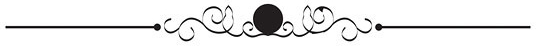
\includegraphics[width=12cm]{../resources/jpg/2.3.functions/border3.jpg}
\end{figure}
\vspace{2\baselineskip}


% ============================== 0091 Theorem 2369a ===============================
\subsection[The ceiling of a floor is that floor.]
    {
        \color{section}Theorem 91. \color{black} The ceiling of a floor is that floor.
    }
\documentclass[preview]{standalone}
\usepackage{amssymb, amsthm}
\usepackage{mathtools}
\usepackage{bm}


\newtheorem{theorem}{Theorem}
\renewcommand\qedsymbol{$\blacksquare$}


\begin{document}


\begin{theorem}[\textbf{2369a}]
    Let \bm{$\lambda$} be a real number. 
    \begin{equation*}
        \bm{
            \Big \lceil \lfloor \lambda \rfloor \Big \rceil 
                = 
            \lfloor \lambda \rfloor
        }
    \end{equation*}
\end{theorem}

\begin{proof}
    By the properties of floor functions, 
    there exists an integer \bm{$\iota$} such that
    \bm{$\lfloor \lambda \rfloor = \iota$}, 
    and by the identity \bm{$\iota$},
    \begin{equation*}
        \bigg \langle \lfloor \lambda \rfloor = \iota \bigg \rangle
            \equiv
        \bigg \langle 
            \Big \lceil \lfloor \lambda \rfloor \Big \rceil
                =
            \big \lceil \iota \big \rceil
        \bigg \rangle
    \end{equation*}
    \bm{$\iota$} is the smallest integer that is greater than or equal to \bm{$\iota$}.
    Therefore, by the definition for the ceiling function 
    \bm{$\lceil \iota \rceil = \iota$}.
    Hence,
    \begin{equation*}
        \bigg \langle \lfloor \lambda \rfloor = \iota \bigg \rangle
            \land
        \bigg \langle 
            \Big \lceil \lfloor \lambda \rfloor \Big \rceil
                =
            \lceil \iota \rceil
                =
            \iota
        \bigg \rangle
    \end{equation*}
    $\therefore \text{\space} \bm{
        \Big \lceil \lfloor \lambda \rfloor \Big \rceil 
            = 
        \lfloor \lambda \rfloor
    }$, by the identity \bm{$\iota$}.
\end{proof}


\end{document}
\pagebreak


% ============================== 0092 Theorem 2369c ===============================
\subsection[A special fact about ceilings.]
    {
        \color{section}Theorem 92. \color{black} A special fact about ceilings.
    }
\documentclass[preview]{standalone}
\usepackage{amssymb, amsthm}
\usepackage{mathtools}
\usepackage{bm}


\newtheorem{theorem}{Theorem}
\renewcommand\qedsymbol{$\blacksquare$}


\begin{document}


\begin{theorem}[\textbf{2369c}]
    Let \bm{$\lambda$} and \bm{$\iota$} be real numbers. 
    \begin{equation*}
        \bm{
            \lceil \lambda \rceil 
                + 
            \lceil \iota \rceil 
                - 
            \lceil \lambda + \iota \rceil 
                = 
            0
                \textbf{, or } 
            1
        }
    \end{equation*}
\end{theorem}

\begin{proof}
    By cases. 
    There are two possible cases. 
    $(i)$ \bm{$\lambda$} or \bm{$\iota$} (or both) are integers, 
    or $(ii)$ neither \bm{$\lambda$} nor \bm{$\iota$} is an integer.
    \\ \\
    \bm{$(i)$} Assume \bm{$\lambda$} or \bm{$\iota$} (or both) are integers. 
    Without loss of generality \bm{$\iota$} is an integer.
    By Theorem 78, 
    \begin{equation*}
        \Big[ 
            \lceil \lambda \rceil 
                + 
            \lceil \iota \rceil 
                - 
            \lceil \lambda + \iota \rceil 
        \Big]
            = 
        \Big[ 
            \lceil \lambda \rceil 
                + 
            \lceil \iota \rceil 
                - 
            \lceil \lambda \rceil 
                + 
            \lceil \iota \rceil 
        \Big]
            = 
        0
    \end{equation*}
    \bm{$(ii)$} Assume neither \bm{$\lambda$} nor \bm{$\iota$} is an integer. 
    There exist real numbers \bm{$\epsilon$} and \bm{$\sigma$} such that 
    \bm{$\lceil \lambda \rceil - \lambda = \epsilon$},
    and \bm{$\lceil \iota \rceil - \iota = \sigma$}. 
    By Theorem 76, 
    \bm{$\lceil \lambda \rceil = \lfloor \lambda \rfloor + 1$}, 
    and \bm{$\lceil \iota \rceil = \lfloor \iota \rfloor + 1$}. 
    Hence, the identities for \bm{$\lambda$}, and \bm{$\iota$} are
    \begin{equation*}
        \bigg[
            \Big \langle \lambda \Big \rangle 
                = 
            \Big\{ 
                \lfloor \lambda \rfloor + \big \langle 1 - \epsilon \big \rangle 
            \Big\}
        \bigg]
            \land
        \bigg[ 
            \Big \langle \iota \Big \rangle 
                = 
            \Big\{ 
                \lfloor \iota \rfloor + \big \langle 1 - \sigma \big \rangle
            \Big\}
        \bigg]
    \end{equation*} 
    Thus, 
    \begin{equation*}
        \bm{
            \lceil \lambda \rceil 
                + 
            \lceil \iota \rceil 
                - 
            \lceil \lambda + \iota \rceil 
        }
            \equiv
    \end{equation*}
    \begin{equation*}
        \Big \langle \lfloor \lambda \rfloor + 1 \Big \rangle 
            + 
        \Big \langle \lfloor \iota \rfloor + 1 \Big \rangle
            - 
        \bigg \lceil
            \Big\{
                \lfloor \lambda \rfloor
                    + 
                \big \langle 1 - \epsilon \big \rangle
            \Big\}
                +
            \Big\{
                \lfloor \iota \rfloor 
                    + 
                \big \langle 1 - \sigma \big \rangle
            \Big\}
        \bigg \rceil
            \equiv
    \end{equation*} 
    \begin{equation*}
        \Big \langle \lfloor \lambda \rfloor + \lfloor \iota \rfloor + 2 \Big \rangle
            - 
        \bigg \lceil
            \lfloor \lambda \rfloor 
                + 
            \lfloor \iota \rfloor 
                + 
            \Big[
                2 
                    - 
                \big \langle \epsilon + \sigma \big \rangle
            \Big]
        \bigg \rceil
    \end{equation*} 
    There are two possible subcases. Either 
    $(a)$ \bm{$\epsilon + \sigma \geq 1$}, 
    or $(b)$ \bm{$\epsilon + \sigma < 1$}.
    \\ \\
    \bm{$(a)$} Assume 
    \bm{$\epsilon + \sigma \ge 1$}. 
    By the additive compatibility law from the order axioms, 
    \bm{$1 \ge 2 - \big \langle \epsilon + \sigma \big \rangle$}. 
    This means that \bm{$1$} is the smallest integer that is greater than or equal to 
    \bm{$2 - \big \langle \epsilon + \sigma \big \rangle$}.
    Thus, by the definition for ceiling functions, 
    and by Theorem 91,
    \begin{equation*}
        \Big[ 
            \lceil \lambda \rceil 
                + 
            \lceil \iota \rceil 
                - 
            \lceil \lambda + \iota \rceil 
        \Big]
            \equiv
        \Big \langle \lfloor \lambda \rfloor + \lfloor \iota \rfloor + 2 \Big \rangle
            - 
        \Big \lceil
            \lfloor \lambda \rfloor 
                + 
            \lfloor \iota \rfloor 
                + 
            1
        \Big \rceil
            = 
        1
    \end{equation*} 
    \bm{$(b)$} Assume 
    \bm{$\epsilon + \sigma < 1$}. 
    By the additive compatibility law from the order axioms,
    \bm{$1 < 2 - \big \langle \epsilon + \sigma \big \rangle$}. 
    This means that $2$ is the smallest integer that is greater than or equal to
    \bm{$2 - \big \langle \epsilon + \sigma \big \rangle$}.
    Thus, by the definition for ceiling functions, 
    and by Theorem 91,
    \begin{equation*}
        \Big[ 
            \lceil \lambda \rceil 
                + 
            \lceil \iota \rceil 
                - 
            \lceil \lambda + \iota \rceil 
        \Big]
            \equiv
        \Big \langle \lfloor \lambda \rfloor + \lfloor \iota \rfloor + 2 \Big \rangle
            - 
        \Big \lceil
            \lfloor \lambda \rfloor 
                + 
            \lfloor \iota \rfloor 
                + 
            2
        \Big \rceil
            = 
        0
    \end{equation*} 
    $\therefore \text{\space} \bm{
        \lceil \lambda \rceil 
            + 
        \lceil \iota \rceil 
            - 
        \lceil \lambda + \iota \rceil 
            = 
        0
            \textbf{, or } 
        1
    }$, whenever \bm{$\lambda$} and \bm{$\iota$} are real 
    numbers.
\end{proof}


\end{document}
\pagebreak


% ============================== 0093 Theorem 2370a ===============================
\begin{figure}[!h]
    \centering
    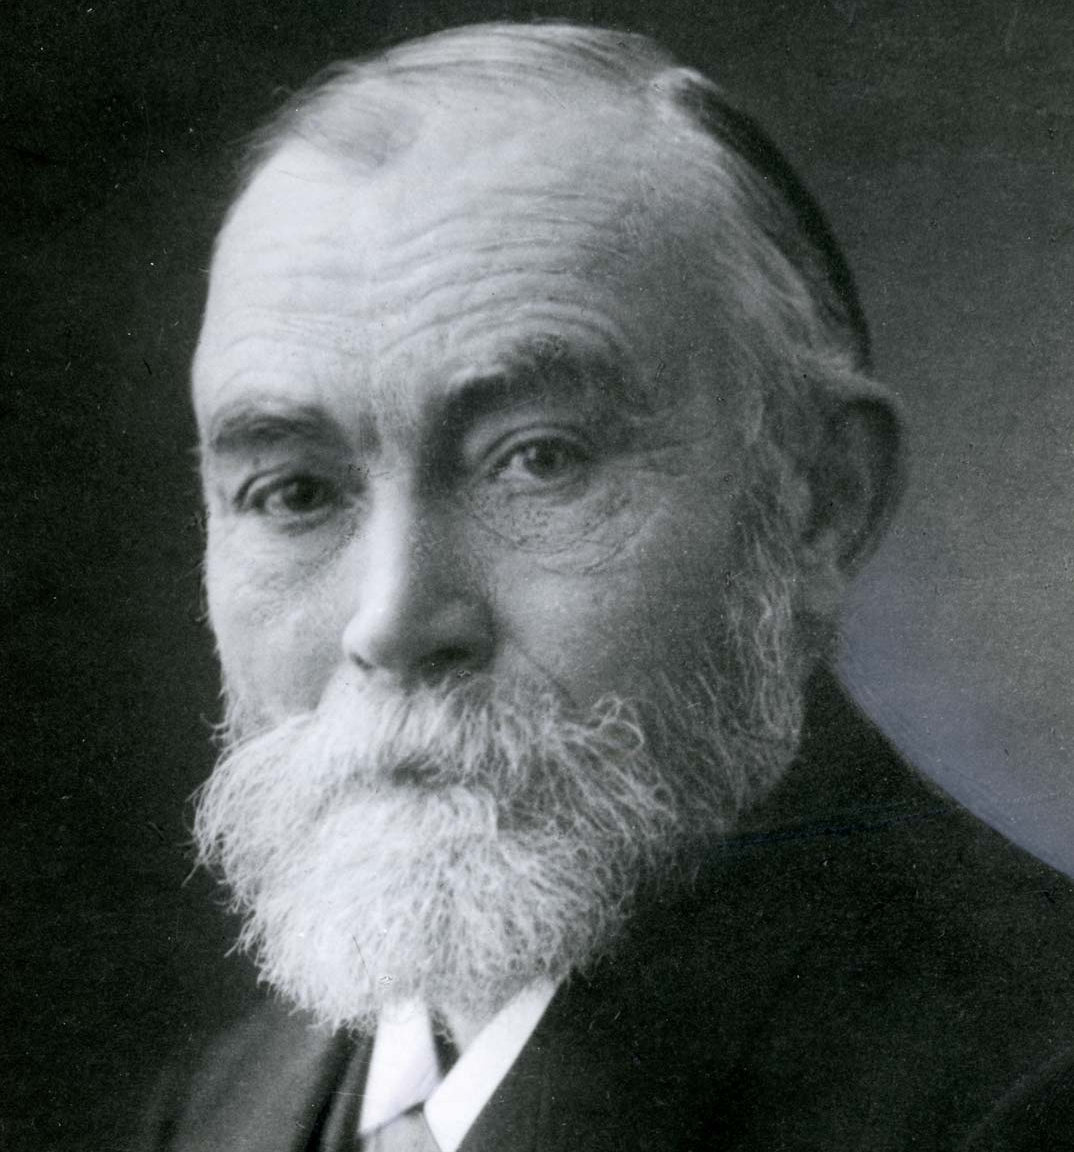
\includegraphics[width=11cm]{../resources/jpg/2.3.functions/frege.jpg}
    \caption*{Gottlob Frege.}
\end{figure}
\subsection[The floor of a ceiling is that ceiling.]
    {
        \color{section}Theorem 93. \color{black} The floor of a ceiling is that ceiling.
    }
\documentclass[preview]{standalone}
\usepackage{amssymb, amsthm}
\usepackage{mathtools}
\usepackage{bm}


\newtheorem{theorem}{Theorem}
\renewcommand\qedsymbol{$\blacksquare$}


\begin{document}


\begin{theorem}[\textbf{2370a}]
    Let \bm{$\lambda$} be a real number. 
    \begin{equation*}
        \bm{
            \Big \lfloor \lceil \lambda \rceil \Big \rfloor 
                = 
            \lceil \lambda \rceil
        }
    \end{equation*}
\end{theorem}

\begin{proof}
    By the properties of ceiling functions,
    there exists an integer \bm{$\iota$} such that
    \bm{$\lceil \lambda \rceil = \iota$}, 
    and by the identity \bm{$\iota$},
    \begin{equation*}
        \bigg \langle \lceil \lambda \rceil = \iota \bigg \rangle
            \equiv
        \bigg \langle 
            \Big \lfloor \lceil \lambda \rceil \Big \rfloor
                =
            \big \lfloor \iota \big \rfloor
        \bigg \rangle
    \end{equation*}
    \bm{$\iota$} is the largest integer that is less than or equal to \bm{$\iota$}.
    Therefore, by the definition for the floor function
    \bm{$\lfloor \iota \rfloor = \iota$}.
    Hence,
    \begin{equation*}
        \bigg \langle \lceil \lambda \rceil = \iota \bigg \rangle
            \land
        \bigg \langle 
            \Big \lfloor \lceil \lambda \rceil \Big \rfloor
                =
            \big \lfloor \iota \big \rfloor
                =
            \iota
        \bigg \rangle
    \end{equation*}
    $\therefore \text{\space} \bm{
        \Big \lfloor \lceil \lambda \rceil \Big \rfloor 
            = 
        \lceil \lambda \rceil
    }$, by the identity \bm{$\iota$}.
\end{proof}


\end{document}
\pagebreak


% ============================== 0094 Theorem 2370c ===============================
\subsection[The ceiling of a quarter.]
    {
        \color{section}Theorem 94. \color{black} The ceiling of a quarter.
    }
\documentclass[preview]{standalone}
\usepackage{amssymb, amsthm}
\usepackage{mathtools}
\usepackage{bm}


\newtheorem{theorem}{Theorem}
\renewcommand\qedsymbol{$\blacksquare$}


\begin{document}


\begin{theorem}[\textbf{2370c}]
    Let \bm{$\iota$} be a real number.
    \begin{equation*}
        \bm{
            \Bigg \lceil \bigg \lceil \frac{\iota}{2} \bigg \rceil \div 2 \Bigg \rceil 
                = 
            \Bigg \lceil \frac{\iota}{4} \Bigg \rceil
        }
    \end{equation*}
\end{theorem}

\begin{proof}
    By cases.
    By the properties for ceiling functions there exists an integer \bm{$\lambda$} such that
    \bm{$\big \lceil \frac{\iota}{4} \big \rceil = \lambda$}, 
    (and by the multiplicative compatibility laws from the order axioms,)
    if and only if
    \begin{equation*}
        \bigg[
            \Big \langle \lambda - 1 \Big \rangle
                < 
            \Big \langle \frac{\iota}{4} \Big \rangle 
                \le 
            \Big \langle \lambda \Big \rangle
        \bigg]
            \equiv
        \bigg[
            \Big \langle 2 \lambda - 2 \Big \rangle
                < 
            \Big \langle \frac{\iota}{2} \Big \rangle 
                \le 
            \Big \langle 2 \lambda \Big \rangle
        \bigg]
    \end{equation*}
    There are two cases to consider. 
    by the definition for the ceiling function, 
    \bm{$\big \lceil \frac{\iota}{2} \big \rceil$} is the integer
    $(i)$ \bm{$2 \lambda$}, or $(ii)$ \bm{$2 \lambda - 1$},
    \\ \\
    \bm{$(i)$} If \bm{$\big \lceil \frac{\iota}{2} \big \rceil$} is \bm{$2 \lambda$},
    then the proof is trivial. By the identity \bm{$\lambda$}, 
    the multiplicative inverse from the field axioms, 
    and by the definition of ceiling functions, 
    \begin{equation*}
        \bigg \lceil \Big \lceil \frac{\iota}{2} \Big \rceil \div 2 \bigg \rceil
            =
        \bigg \langle \big \lceil 2 \lambda \div 2 \big \rceil \bigg \rangle
            =
        \bigg \langle \big \lceil \lambda \big \rceil \bigg \rangle
            =
        \bigg \langle \lambda \bigg \rangle
    \end{equation*}
    \bm{$(ii)$} Suppose \bm{$\big \lceil \frac{\iota}{2} \big \rceil = 2 \lambda - 1$}.
    By the properties for ceiling functions,
    and by the law of transitivity from the order axioms,
    \begin{equation*}
        \bigg[
            \Big \langle 2 \lambda - 2 \Big \rangle
                < 
            \Big \langle \Big \lceil \frac{\iota}{2} \Big \rceil \Big \rangle
                \le 
            \Big \langle 2 \lambda - 1\Big \rangle
        \bigg]
            \rightarrow
        \bigg[
            \Big \langle 2 \lambda - 2 \Big \rangle
                < 
            \Big \langle \Big \lceil \frac{\iota}{2} \Big \rceil \Big \rangle
                \le 
            \Big \langle 2 \lambda \Big \rangle
        \bigg]
    \end{equation*}
    Thus, by the multiplicative compatibility law from the order axioms,
    \begin{equation*}
        \bigg[
            \Big \langle 2 \lambda - 2 \Big \rangle
                < 
            \Big \langle \Big \lceil \frac{\iota}{2} \Big \rceil \Big \rangle
                \le 
            \Big \langle 2 \lambda \Big \rangle
        \bigg]
            \equiv
        \bigg[
            \Big \langle \lambda - 1 \Big \rangle
                < 
            \Big \langle \Big \lceil \frac{\iota}{2} \Big \rceil \div 2 \Big \rangle
                \le 
            \Big \langle \lambda \Big \rangle
        \bigg]
    \end{equation*}
    By the properties for ceiling functions, 
    $\big \lceil \big \lceil \frac{\iota}{2} \big \rceil \div 2 \big \rceil = \lambda$.
    \\ \\
    $\therefore \text{\space} \bm{
        \bigg \lceil \Big \lceil \frac{\iota}{2} \Big \rceil \div 2 \bigg \rceil 
            = 
        \Big \lceil \frac{\iota}{4} \Big \rceil
    }$
\end{proof}


\end{document}
\vspace{1.5\baselineskip}
\begin{figure}[!h]
    \centering
    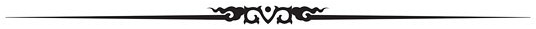
\includegraphics[width=12cm]{../resources/jpg/2.3.functions/border4.jpg}
\end{figure}
\pagebreak


% ============================== 0095 Theorem 2370e ===============================
\subsection[A special fact about floors.]
    {
        \color{section}Theorem 95. \color{black} A special fact about floors.
    }
\documentclass[preview]{standalone}
\usepackage{amssymb, amsthm}
\usepackage{mathtools}
\usepackage{bm}


\newtheorem{theorem}{Theorem}
\renewcommand\qedsymbol{$\blacksquare$}


\begin{document}


\begin{theorem}[\textbf{2370e}]
    Let \bm{$\lambda$}, and \bm{$\iota$} be real numbers.
    \begin{equation*}
        \bm{
            \big \lfloor \lambda \big \rfloor 
                + 
            \big \lfloor \iota \big \rfloor  
                + 
            \big \lfloor \lambda + \iota \big \rfloor 
                \le 
            \big \lfloor 2 \lambda \big \rfloor 
                + 
            \big \lfloor 2 \iota \big \rfloor
        }
    \end{equation*}
\end{theorem}

\begin{proof}
    By cases.
    There exist real numbers \bm{$\epsilon$} and \bm{$\sigma$} such that
    \bm{$\lambda - \lfloor \lambda \rfloor = \epsilon$}. 
    By the property for floor functions,
    \bm{$\lfloor \lambda \rfloor = \lambda - \epsilon$},
    if and only if
    \begin{equation*}
        \Big \langle \lambda - \epsilon \Big \rangle
            \leq 
        \Big \langle \lambda \Big \rangle
            < 
        \Big \langle \lambda - \epsilon + 1 \Big \rangle
    \end{equation*}
    Without loss of generality with respect to \bm{$\iota$}, 
    by additive compatibility from the order axioms,
    there exists an integer 
    \bm{$
        \lfloor \lambda + \iota \rfloor 
            = 
        \big \langle \lambda - \epsilon \big \rangle
            +
        \big \langle \iota - \sigma \big \rangle$},
    if and only if
    \begin{equation*}
        \Big \langle
            \lambda - \epsilon
                + 
            \iota - \sigma
        \Big \rangle
            \leq 
        \Big \langle \lambda + \iota \Big \rangle
            < 
        \Big \langle
            \lambda - \epsilon
                + 
            \iota - \sigma
                + 
            1
        \Big \rangle
    \end{equation*}
    Thus, by the identities for the floor of \bm{$\lambda$},
    the floor of \bm{$\iota$}, 
    and the floor of the sum of \bm{$\lambda$} and \bm{$\iota$},
    we deduce 
    \begin{equation*}
        \big \lfloor \lambda \big \rfloor
            +
        \big \lfloor \iota \big \rfloor
            +
        \big \lfloor \lambda + \iota \big \rfloor
            =
        \Big[
            \big \langle \lambda - \epsilon \big \rangle
                +
            \big \langle \iota - \sigma \big \rangle
                +
            \big \langle \lambda - \epsilon + \iota - \sigma \big \rangle
        \Big]
            =
    \end{equation*}
    \begin{equation*}
        2 \big \langle \lambda + \iota \big \rangle 
            -
        2 \big \langle \epsilon + \sigma \big \rangle
    \end{equation*}
    Now, by multiplicative compatibility, 
    and transitivity from the order axioms,
    \begin{equation*}
        \Big \langle \lambda - \epsilon \Big \rangle
            \leq 
        \Big \langle \lambda \Big \rangle
            < 
        \Big \langle \lambda - \epsilon + 1 \Big \rangle
            \equiv
        \Big \langle 2 \lambda - 2\epsilon \Big \rangle
            \leq 
        \Big \langle 2 \lambda \Big \rangle
            < 
        \Big \langle 2 \lambda - 2\epsilon + 2 \Big \rangle
            \equiv
    \end{equation*}
    \begin{equation*}
        \Big \langle 2 \big[ \lambda - \epsilon \big] \Big \rangle
            \leq
        \Big \langle 2 \lambda \Big \rangle
            \leq
        \Big \langle 2 \big[ \lambda - \epsilon \big] + 1 \Big \rangle
    \end{equation*}
    So \bm{$
        \big \lfloor 2 \lambda \big \rfloor
    $}
    is the integer
    $(i)$ \bm{$
        2 \big \langle \lambda - \epsilon \big \rangle
    $}, 
    or $(ii)$ \bm{$
        2 \big \langle \lambda - \epsilon \big \rangle + 1
    $}, by the properties for the floor function.
    \\ \\
    \bm{$(i)$} Let \bm{$
        \big \lfloor 2 \lambda \big \rfloor 
            = 
        2 \big \langle \lambda - \epsilon \big \rangle
    $}. 
    Without loss of generality with respect to \bm{$\iota$},
    \begin{equation*}
        \Big \{ 
            \big \lfloor 2 \lambda \big \rfloor 
                + 
            \big \lfloor 2 \iota \big \rfloor
        \Big \}
            =
        \Big \{
            2 \big \langle \lambda - \epsilon \big \rangle 
                + 
            2 \big \langle \iota - \sigma \big \rangle
        \Big \}
            =
        \Big \{
            2 \big \langle \lambda + \iota \big \rangle
                - 
            2 \big \langle \epsilon + \sigma \big \rangle
        \Big \}
            =
    \end{equation*}
    \begin{equation*}
        \Big \{
            \big \lfloor \lambda \big \rfloor
                +
            \big \lfloor \iota \big \rfloor
                +
            \big \lfloor \lambda + \iota \big \rfloor
        \Big \}
    \end{equation*}
    \bm{$(ii)$} Let \bm{$
    \big \lfloor 2 \lambda \big \rfloor
        = 
    2 \big \langle \lambda - \epsilon \big \rangle + 1
    $}.
    Without loss of generality with respect to \bm{$\iota$},
    \begin{equation*}
        \Big \{
            \big \lfloor 2 \lambda \big \rfloor 
                + 
            \big \lfloor 2 \iota \big \rfloor
        \Big \}
            =
        \Big \{
            2 \big \langle \lambda - \epsilon \big \rangle + 1 
                + 
            2 \big \langle \iota - \sigma \big \rangle + 1
        \Big \}
            =
        \Big \{
            2 \big \langle \lambda + \iota + 1 \big \rangle 
                - 
            2 \big \langle \epsilon + \sigma \big \rangle
        \Big \}
    \end{equation*}
    \begin{equation*}
            >
        \Big\{
            \big \lfloor \lambda \big \rfloor
                +
            \big \lfloor \iota \big \rfloor
                +
            \big \lfloor \lambda + \iota \big \rfloor
        \Big\}
    \end{equation*}
    $\therefore \text{\space} \bm{
        \big \lfloor \lambda \rfloor 
            + 
        \big \lfloor \iota \rfloor  
            + 
        \big \lfloor \lambda + \iota \rfloor 
            \le 
        \big \lfloor 2 \lambda \rfloor 
            + 
        \big \lfloor 2 \iota \rfloor 
    }$.
\end{proof}


\end{document}
\pagebreak


% ============================== 0096 Theorem 2371a ===============================
\subsection[The floor of a square root.]
    {
        \color{section}Theorem 96. \color{black} The floor of a square root.
    }
\documentclass[preview]{standalone}
\usepackage{amssymb, amsthm}
\usepackage{mathtools}
\usepackage{bm}


\newtheorem{theorem}{Theorem}
\renewcommand\qedsymbol{$\blacksquare$}


\begin{document}


\begin{theorem}[\textbf{2371a}]
    Let \bm{$\lambda$} be a positive real number. 
    \begin{equation*}
        \bm{
            \bigg \lfloor 
                \sqrt{ \strut \big \lfloor \lambda \big \rfloor } 
            \bigg \rfloor 
                = 
            \bigg \lfloor \sqrt{ \strut \lambda} \bigg \rfloor
        }
    \end{equation*}
\end{theorem}


\begin{proof}
    By the properties for floor functions,
    there exists an integer 
    \bm{$
        \big \lfloor \sqrt{ 
            \lfloor \lambda \rfloor 
        } \big \rfloor
    $} such that 
    \bm{$
        \big \lfloor \sqrt{ \lambda} \big \rfloor
            = 
        \big \lfloor \sqrt{ 
            \lfloor \lambda \rfloor 
        } \big \rfloor 
    $},
    if and only if
    \begin{equation*}
        \bigg \langle 
            \bigg \lfloor 
                \sqrt{ 
                    \big \lfloor \lambda \big \rfloor
                }
            \bigg \rfloor
        \bigg \rangle
            \leq
        \bigg \langle
            \sqrt{ \strut \lambda }
        \bigg \rangle
            <
        \bigg \langle 
            \bigg \lfloor 
                \sqrt{ 
                    \big \lfloor \lambda \big \rfloor
                }
            \bigg \rfloor
                +
            1
        \bigg \rangle
    \end{equation*}
    By the multiplicative compatibility law from the order axioms, that is
    \begin{equation*}
        \bigg \langle 
            \bigg \lfloor 
                \sqrt{ 
                    \big \lfloor \lambda \big \rfloor
                }
            \bigg \rfloor
        \bigg \rangle
            ^2
            \leq
        \bigg \langle
            \lambda
        \bigg \rangle
            <
        \bigg \langle 
            \bigg \lfloor 
                \sqrt{ 
                    \big \lfloor \lambda \big \rfloor
                }
            \bigg \rfloor
                +
            1
        \bigg \rangle
        ^2
    \end{equation*}
    \bm{$\big \lfloor \lambda \big \rfloor$} 
    is the largest integer that is less than or equal \bm{$\lambda$},
    so by the definition of the floor function, 
    \bm{$\big \lfloor \lambda \big \rfloor \leq \lambda$}. 
    Also,
    \bm{$\big \lfloor \sqrt{ \lfloor \lambda \rfloor } \big \rfloor ^2$}
    is an integer by the defintion of floor functions,
    since integers are closed under multiplication. 
    Hence,
    \bm{$
        \big \lfloor \sqrt{ \lfloor \lambda \rfloor } \big \rfloor ^2
            \leq
        \big \lfloor \lambda \big \rfloor
    $}.
    So by the transitivity law from the order axioms,
    \begin{equation*}
        \bigg \langle 
            \bigg \lfloor 
                \sqrt{ 
                    \big \lfloor \lambda \big \rfloor
                }
            \bigg \rfloor
        \bigg \rangle
            ^2
            \leq
        \bigg \langle
            \big \lfloor \lambda \big \rfloor
        \bigg \rangle
            \leq
        \bigg \langle
            \lambda
        \bigg \rangle
            <
        \bigg \langle 
            \bigg \lfloor 
                \sqrt{ 
                    \big \lfloor \lambda \big \rfloor
                }
            \bigg \rfloor
                +
            1
        \bigg \rangle
            ^2
            \equiv
    \end{equation*}
    \begin{equation*}
        \bigg \langle 
            \bigg \lfloor 
                \sqrt{ 
                    \big \lfloor \lambda \big \rfloor
                }
            \bigg \rfloor
        \bigg \rangle
            ^2
            \leq
        \bigg \langle
            \big \lfloor \lambda \big \rfloor
        \bigg \rangle
            <
        \bigg \langle 
            \bigg \lfloor 
                \sqrt{ 
                    \big \lfloor \lambda \big \rfloor
                }
            \bigg \rfloor
                +
            1
        \bigg \rangle
            ^2
    \end{equation*}
    By the multiplicative compatibility law from the order axioms,
    the following is an equivalent statement,
    \begin{equation*}
        \bigg \langle 
            \bigg \lfloor 
                \sqrt{ 
                    \big \lfloor \lambda \big \rfloor
                }
            \bigg \rfloor
        \bigg \rangle
            \leq
        \bigg \langle
            \sqrt{ \strut \big \lfloor \lambda \big \rfloor }
        \bigg \rangle
            <
        \bigg \langle 
            \bigg \lfloor 
                \sqrt{ 
                    \big \lfloor \lambda \big \rfloor
                }
            \bigg \rfloor
                +
            1
        \bigg \rangle
    \end{equation*}
    $\therefore \text{\space} \bm{
        \bigg \lfloor 
            \sqrt{ \strut \big \lfloor \lambda \big \rfloor } 
        \bigg \rfloor 
            = 
        \bigg \lfloor \sqrt{ \strut \lambda} \bigg \rfloor
    }$, by the properties of floor functions.
\end{proof}


\end{document}
\begin{figure}[!h]
    \centering
    
\includegraphics[width=3cm]{../resources/jpg/2.3.functions/symbol6.jpg}
\end{figure}
\pagebreak


% ============================== 0097 Theorem 2371b ===============================
\begin{figure}[!h]
    \centering
    
\includegraphics[width=14cm]{../resources/jpg/2.3.functions/border5.jpg}
\end{figure}
\subsection[The ceiling of a square root.]
    {
        \color{section}Theorem 97. \color{black} The ceiling of a square root.
    }
\documentclass[preview]{standalone}
\usepackage{amssymb, amsthm}
\usepackage{mathtools}
\usepackage{bm}


\newtheorem{theorem}{Theorem}
\renewcommand\qedsymbol{$\blacksquare$}


\begin{document}


\begin{theorem}[\textbf{2371b}]
    Let \bm{$\lambda$} be a positive real number.
    \begin{equation*}
        \bm{
            \bigg \lceil 
                \sqrt{ \strut \big \lceil \lambda \big \rceil }
            \bigg \rceil 
                = 
            \bigg \lceil \sqrt{ \strut \lambda } \bigg \rceil
        }
    \end{equation*}
\end{theorem}

\begin{proof}
    By the properties for ceiling functions,
    there exists an integer
    \bm{$\big \lceil \sqrt{ \lceil \lambda \rceil} \big \rceil$}
    such that
    \bm{$
        \big \lceil \sqrt{ \lambda } \big \rceil
            =
        \big \lceil \sqrt{ \lceil \lambda \rceil} \big \rceil$
    },
    if and only if
    \begin{equation*}
        \bigg \langle
            \bigg \lceil
                \sqrt{ \strut \big \lceil \lambda \big \rceil }
            \bigg \rceil
                -
            1
        \bigg \rangle
            <
        \bigg \langle
            \sqrt{ \strut \lambda }
        \bigg \rangle
            \leq
        \bigg \langle
            \bigg \lceil
                \sqrt{ \strut \big \lceil \lambda \big \rceil }
            \bigg \rceil
        \bigg \rangle
    \end{equation*}
    By the multiplicative compatibility law from the order axioms, that is
    \begin{equation*}
        \bigg \langle
            \bigg \lceil
                \sqrt{ \strut \big \lceil \lambda \big \rceil }
            \bigg \rceil
                -
            1
        \bigg \rangle
            ^2
            <
        \bigg \langle
            \lambda
        \bigg \rangle
            \leq
        \bigg \langle
            \bigg \lceil
                \sqrt{ \strut \big \lceil \lambda \big \rceil }
            \bigg \rceil
        \bigg \rangle
            ^2
    \end{equation*}
    \bm{$\big \lceil \lambda \big \rceil$} is the smallest integer that is greater than or equal to \bm{$\lambda$},
    so by the definition of the ceiling function, 
    \bm{$\lambda \leq \big \lceil \lambda \big \rceil$}.
    Also, 
    \bm{$\big \lceil \sqrt{ \lceil \lambda \rceil} \big \rceil ^2$}
    is an integer by the definition of floor functions,
    since integers are closed under multiplication.
    Hence,
    \bm{$
        \big \lceil \lambda \big \rceil
            \leq
        \big \lceil \sqrt{ \lceil \lambda \rceil} \big \rceil ^2
    $}.
    So by the transitivity law from the order axioms,
    \begin{equation*}
        \bigg \langle
            \bigg \lceil
                \sqrt{ \strut \big \lceil \lambda \big \rceil }
            \bigg \rceil
                -
            1
        \bigg \rangle
            ^2
            <
        \bigg \langle
            \lambda
        \bigg \rangle
            \leq
        \bigg \langle
            \big \lceil \lambda \big \rceil
        \bigg \rangle
            \leq
        \bigg \langle
            \bigg \lceil
                \sqrt{ \strut \big \lceil \lambda \big \rceil }
            \bigg \rceil
        \bigg \rangle
            ^2
            \equiv
    \end{equation*}
    \begin{equation*}
        \bigg \langle
            \bigg \lceil
                \sqrt{ \strut \big \lceil \lambda \big \rceil }
            \bigg \rceil
                -
            1
        \bigg \rangle
            ^2
            <
        \bigg \langle
            \big \lceil \lambda \big \rceil
        \bigg \rangle
            \leq
        \bigg \langle
            \bigg \lceil
                \sqrt{ \strut \big \lceil \lambda \big \rceil }
            \bigg \rceil
        \bigg \rangle
            ^2
    \end{equation*}
    By the multiplicative compatibility law from the order axioms,
    the following is an equivalent statement,
    \begin{equation*}
        \bigg \langle
            \bigg \lceil
                \sqrt{ \strut \big \lceil \lambda \big \rceil }
            \bigg \rceil
                -
            1
        \bigg \rangle
            <
        \bigg \langle
            \sqrt{ \strut \big \lceil \lambda \big \rceil }
        \bigg \rangle
            \leq
        \bigg \langle
            \bigg \lceil
                \sqrt{ \strut \big \lceil \lambda \big \rceil }
            \bigg \rceil
        \bigg \rangle
    \end{equation*}
    $\therefore \text{\space} \bm{
        \bigg \lceil 
            \sqrt{ \strut \big \lceil \lambda \big \rceil }
        \bigg \rceil 
            = 
        \bigg \lceil \sqrt{ \strut \lambda } \bigg \rceil
    }$, by the properties of ceiling functions.
\end{proof}


\end{document}
\pagebreak


% ============================== 0098 Theorem 2372 ================================
\subsection[The floor of integers divisible by 3.]
    {
        \color{section}Theorem 98. \color{black} The floor of integers divisible by 3.
    }
\documentclass[preview]{standalone}
\usepackage{amssymb, amsthm}
\usepackage{mathtools}
\usepackage{bm}


\newtheorem{theorem}{Theorem}
\renewcommand\qedsymbol{$\blacksquare$}


\begin{document}


\begin{theorem}[\textbf{2372}]
    Let \bm{$\lambda$} be a real number, such that
    \bm{$\big \lfloor \lambda \big \rfloor + \epsilon = \lambda$}.
    \begin{equation*}
        \bm{
            \bigg \lfloor 3 \lambda \bigg \rfloor
                = 
            \bigg \lfloor \lambda \bigg \rfloor
                + 
            \bigg \lfloor \lambda + \frac{1}{3} \bigg \rfloor
                + 
            \bigg \lfloor \lambda + \frac{2}{3} \bigg \rfloor
        }
    \end{equation*}
\end{theorem}

\begin{proof}
    By cases. By Lemma 9, it is sufficent to prove
    \begin{equation*}
        \bigg \lfloor 3 \epsilon \bigg \rfloor
            =
        \Bigg \langle 
            \mathrm{A} 
                = 
            \bigg \lfloor \epsilon \bigg \rfloor 
        \Bigg \rangle
            +
        \Bigg \langle
            \Lambda
                = 
            \bigg \lfloor \epsilon + \frac{1}{3} \bigg \rfloor 
        \Bigg \rangle
            +
        \Bigg \langle
            \Delta
                = 
            \bigg \lfloor \epsilon + \frac{2}{3} \bigg \rfloor
        \Bigg \rangle
    \end{equation*}
    Let \bm{$p$} be the propostion: \bm{$\Delta \geq \Lambda \geq \mathrm{A} \geq 0$}.
    The proof for which is trivial.
    There are three cases:
    \\ \\
    \indent \indent \bm{$(i)$} \space \space
    $
        \Big \langle 0 \Big \rangle 
            \le 
        \Big \langle \epsilon \Big \rangle
            < 
        \Big \langle \frac{1}{3} \Big \rangle
    $
    \\ \\
    \indent \indent \bm{$(ii)$} \space
    $
        \Big \langle \frac{1}{3} \Big \rangle 
            \le 
        \Big \langle \epsilon \Big \rangle
            < 
        \Big \langle \frac{2}{3} \Big \rangle
    $ 
    \\ \\
    \indent \indent \bm{$(iii)$}
    $ 
        \Big \langle \frac{2}{3} \Big \rangle 
            \le 
        \Big \langle \epsilon \Big \rangle 
            < 
        \Big \langle 1 \Big \rangle
    $
    \\ \\
    \bm{$(i)$}
    Since \bm{$p$}, 
    \bm{$\Delta$} is sufficient for inferring \bm{$\mathrm{A}$}, 
    and \bm{$\Lambda$} in this case.
    By the additive compatibility law from the order axioms, 
    and by the law of transitivity from the order axioms,
    \begin{equation*}
        \bigg[
            \bigg \langle \frac{0}{3} + \frac{2}{3} \bigg \rangle
                \leq 
            \bigg \langle \epsilon + \frac{2}{3} \bigg \rangle 
                < 
            \bigg \langle \frac{1}{3} + \frac{2}{3} \bigg \rangle
        \bigg]
            \equiv
        \bigg[
            \bigg \langle 0 \bigg \rangle
                \leq 
            \bigg \langle \epsilon + \frac{2}{3} \bigg \rangle 
                < 
            \bigg \langle 1 \bigg \rangle
        \bigg]
    \end{equation*}
    Thus, \bm{$\Delta = 0$}, by the properties of floor functions. 
    Hence, \bm{$\mathrm{A} + \Lambda + \Delta = 0$}, by \bm{$p$}. 
    Also, by the multiplicative compatibility law from the order axioms,
    and by the properties of floor functions,
    \begin{equation*}
        \bigg[
            \bigg \langle 3 \cdot 0 \bigg \rangle
                \leq
            \bigg \langle 3 \cdot \epsilon \bigg \rangle
                <
            \bigg \langle 3 \cdot \frac{1}{3} \bigg \rangle
        \bigg]
            \equiv
        \bigg[
            \big \lfloor 3 \epsilon \big \rfloor
                =
            0
        \bigg]
    \end{equation*}
    $\therefore \text{\space} \bm{
        \big \lfloor 3 \epsilon \big \rfloor
            =
        \mathrm{A} + \Lambda + \Delta
    }$, by the identity \bm{$0$}, in this case.
    \\ \\
    \bm{$(ii)$}
    Since \bm{$p$}, \bm{$\Lambda$} is sufficent for inferring \bm{$\mathrm{A}$} in this case.
    By the additive compatibility law from the order axioms,
    and by the law of transitivity,
    \begin{equation*}
        \bigg[
            \bigg \langle \frac{1}{3} + \frac{1}{3} \bigg \rangle
                \leq 
            \bigg \langle \epsilon + \frac{1}{3} \bigg \rangle 
                < 
            \bigg \langle \frac{2}{3} + \frac{1}{3} \bigg \rangle
        \bigg]
            \equiv
        \bigg[
            \bigg \langle 0 \bigg \rangle
                \leq 
            \bigg \langle \epsilon + \frac{1}{3} \bigg \rangle 
                < 
            \bigg \langle 1 \bigg \rangle
        \bigg]
    \end{equation*}
    Thus, \bm{$\Lambda = 0$}, by the properties of floor functions.
    Hence, \bm{$\mathrm{A} + \Lambda = 0$}, by \bm{$p$}. 
    Now, for \bm{$\Delta$}, 
    by the additive compatibility law from the order axioms,
    and by the law of transitivity from the order axioms,
    \pagebreak
    \begin{equation*}
        \bigg[
            \bigg \langle \frac{1}{3} + \frac{2}{3} \bigg \rangle
                \leq 
            \bigg \langle \epsilon + \frac{2}{3} \bigg \rangle 
                < 
            \bigg \langle \frac{2}{3} + \frac{2}{3} \bigg \rangle
        \bigg]
            \equiv
        \bigg[
            \bigg \langle 1 \bigg \rangle
                \leq 
            \bigg \langle \epsilon + \frac{2}{3} \bigg \rangle 
                < 
            \bigg \langle 1 + 1 \bigg \rangle
        \bigg]
    \end{equation*}
    Thus, \bm{$\Delta = 1$}, by the properties of floor functions. 
    Hence, \bm{$\mathrm{A} + \Lambda + \Delta = 1$}.
    Also, by the multiplicative compatibility law from the order axioms,
    and by the properties of floor functions,
    \begin{equation*}
        \bigg[
            \bigg \langle 3 \cdot \frac{1}{3} \bigg \rangle
                \leq
            \bigg \langle 3 \cdot \epsilon \bigg \rangle
                <
            \bigg \langle 3 \cdot \frac{2}{3} \bigg \rangle
        \bigg]
            \equiv
    \end{equation*}
    \begin{equation*}
        \bigg[
            \Big \langle 1 \Big \rangle
                \leq
            \Big \langle 3 \epsilon \Big \rangle
                <
            \Big \langle 1 + 1 \Big \rangle
        \bigg]
            \equiv
        \bigg[
            \big \lfloor 3 \epsilon \big \rfloor
                =
            1
        \bigg]
    \end{equation*}
    $\therefore \text{\space} \bm{
        \lfloor 3 \epsilon \rfloor
            =
        \mathrm{A} + \Lambda + \Delta
    }$, by the identity \bm{$1$}, in this case.
    \\ \\
    \bm{$(iii)$} 
    \bm{$\mathrm{A} = 0$} can be inferred from the law of transitivity from the order axioms,
    and by the properties of floor functions, in this case.
    For \bm{$\Lambda$},
    by the additive compatibility law from the order axioms,
    and by the law of transitivity from the order axioms,
    \begin{equation*}
        \bigg[
            \bigg \langle \frac{2}{3} + \frac{1}{3} \bigg \rangle
                \leq 
            \bigg \langle \epsilon + \frac{1}{3} \bigg \rangle 
                < 
            \bigg \langle \frac{3}{3} + \frac{1}{3} \bigg \rangle
        \bigg]
            \equiv
        \bigg[
            \bigg \langle 1 \bigg \rangle
                \leq 
            \bigg \langle \epsilon + \frac{1}{3} \bigg \rangle 
                < 
            \bigg \langle 1 + 1 \bigg \rangle
        \bigg]
    \end{equation*}
    Thus, \bm{$\Lambda = 1$}, 
    by the properties of floor functions.
    For \bm{$\Delta$},
    by the additive compatibility law from the order axioms,
    and by the law of transitivity from the order axioms,
    \begin{equation*}
        \bigg[
            \bigg \langle \frac{2}{3} + \frac{2}{3} \bigg \rangle
                \leq 
            \bigg \langle \epsilon + \frac{2}{3} \bigg \rangle 
                < 
            \bigg \langle \frac{3}{3} + \frac{2}{3} \bigg \rangle
        \bigg]
            \equiv
        \bigg[
            \bigg \langle 1 \bigg \rangle
                \leq 
            \bigg \langle \epsilon + \frac{2}{3} \bigg \rangle 
                < 
            \bigg \langle 1 + 1 \bigg \rangle
        \bigg]
    \end{equation*}
    Thus, \bm{$\Delta = 1$}, 
    by the properties of floor functions.
    Hence, \bm{$\mathrm{A} + \Lambda + \Delta = 2$}.
    Also, by the multiplicative compatibility law from the order axioms,
    and by the properties of floor functions,
    \begin{equation*}
        \bigg[
            \bigg \langle 3 \cdot \frac{2}{3} \bigg \rangle
                \leq
            \bigg \langle 3 \cdot \epsilon \bigg \rangle
                <
            \bigg \langle 3 \cdot 1 \bigg \rangle
        \bigg]
            \equiv
    \end{equation*}
    \begin{equation*}
        \bigg[
            \bigg \langle 2 \bigg \rangle
                \leq
            \bigg \langle 3 \epsilon \bigg \rangle
                <
            \bigg \langle 2 + 1 \bigg \rangle
        \bigg]
            \equiv
        \bigg[
            \big \lfloor 3 \epsilon \big \rfloor
                =
            2
        \bigg]
    \end{equation*}
    $\therefore \text{\space} \bm{
        \lfloor 3 \epsilon \rfloor
            =
        \mathrm{A} + \Lambda + \Delta
    }$, by the identity \bm{$2$}, in this case.
    \\ \\
    This completes the proof.
\end{proof}


\end{document}
\sep
\pagebreak


\section{Lemmas}
% ================================ 0006L Lemma 2301 =================================
\subsection[Lemma 6]{\color{section}Lemma 6}
\documentclass[preview]{standalone}
\usepackage{amssymb, amsthm}
\usepackage{mathtools}
\usepackage{bm}


\newtheorem{lemma}{Lemma}
\renewcommand\qedsymbol{$\blacksquare$}


\begin{document}


\begin{lemma}[\textbf{2301}]
    Let \bm{$\lambda$} be a real number, 
    and let \bm{$\zeta$} be an integer. 
    \begin{equation*}
        \bm{\lfloor \lambda + \zeta \rfloor 
            =
        \lfloor \lambda \rfloor + \zeta}
    \end{equation*}
\end{lemma}

\begin{proof}
    Given \bm{$\lfloor \lambda \rfloor$}, by the properties for floor functions we have
    \begin{equation*}
        \Big \langle \lfloor \lambda \rfloor \Big \rangle
            \leq
        \Big \langle \lambda \Big \rangle
            <
        \Big \langle \lfloor \lambda \rfloor + 1 \Big \rangle
    \end{equation*}
    By the additive compatibility law from the order axioms, that is
    \begin{equation*}
        \Big \langle \lfloor \lambda \rfloor + \zeta \Big \rangle
            \leq
        \Big \langle \lambda + \zeta \Big \rangle
            < 
        \Big \langle \big[ \lfloor \lambda \rfloor + \zeta \big] + 1 \Big \rangle
    \end{equation*} 
    $\therefore \text{\space} \bm{
    \lfloor \lambda + \zeta \rfloor = \lfloor \lambda \rfloor + \zeta$},
    by the properties for floor functions.    
\end{proof}


\end{document}
\sep


% ================================ 0007L Lemma 2302 =================================
\subsection[Lemma 7]{\color{section}Lemma 7}
\documentclass[preview]{standalone}
\usepackage{amssymb, amsthm}
\usepackage{mathtools}
\usepackage{bm}


\newtheorem{lemma}{Lemma}
\renewcommand\qedsymbol{$\blacksquare$}


\begin{document}


\begin{lemma}[\textbf{2302}]
    Let \bm{$\lambda$} be a real number, 
    such that \bm{$\big \lfloor \lambda \big \rfloor + \epsilon = \lambda$}.
    \begin{equation*}
        \bm{
            \Bigg\{
                \bigg \lfloor \lambda \bigg \rfloor 
                    + 
                \bigg \lfloor \lambda + \frac{1}{3} \bigg \rfloor 
                    + 
                \bigg \lfloor \lambda + \frac{2}{3} \bigg \rfloor
            \Bigg\}
                =
            \Bigg\{
                3 \lambda - 3 \epsilon 
                    +
                \bigg \lfloor \epsilon \bigg \rfloor 
                    +
                \bigg \lfloor \epsilon + \frac{1}{3} \bigg \rfloor
                    +
                \bigg \lfloor \epsilon + \frac{2}{3} \bigg \rfloor            
            \Bigg\}
        }
    \end{equation*}
\end{lemma}

\begin{proof}
    Given the real number \bm{$\lambda$}, 
    by the properties for floor functions
    there exists a real number \bm{$\epsilon$}
    and an integer \bm{$\lambda - \epsilon$} such that 
    \bm{$\lfloor \lambda \rfloor = \lambda - \epsilon$}.
    Thus, \bm{$\lambda = \lambda - \epsilon + \epsilon$}.
    By the identity \bm{$\lambda$},
    \begin{equation*}
        \bigg \lfloor \lambda \bigg \rfloor 
            + 
        \bigg \lfloor \lambda + \frac{1}{3} \bigg \rfloor 
            + 
        \bigg \lfloor \lambda + \frac{2}{3} \bigg \rfloor
            =
    \end{equation*}
    \begin{equation*}
        \bigg \lfloor \lambda - \epsilon + \epsilon \bigg \rfloor 
            + 
        \bigg \lfloor \lambda - \epsilon + \epsilon + \frac{1}{3} \bigg \rfloor 
            + 
        \bigg \lfloor \lambda - \epsilon + \epsilon + \frac{2}{3} \bigg \rfloor
    \end{equation*}
    Since \bm{$\lambda - \epsilon$} is an integer, by Lemma 2301 that is
    \begin{equation*}
        \bigg \langle \lambda - \epsilon \bigg \rangle + \bigg \lfloor \epsilon \bigg \rfloor 
            + 
        \bigg \langle \lambda - \epsilon \bigg \rangle + \bigg \lfloor \epsilon + \frac{1}{3} \bigg \rfloor 
            + 
        \bigg \langle \lambda - \epsilon \bigg \rangle + \bigg \lfloor \epsilon + \frac{2}{3} \bigg \rfloor
            =
    \end{equation*}
    \begin{equation*}
        \bigg \langle 3 \lambda - 3 \epsilon \bigg \rangle
            + 
        \bigg \lfloor \epsilon \bigg \rfloor 
            + 
        \bigg \lfloor \epsilon + \frac{1}{3} \bigg \rfloor 
            + 
        \bigg \lfloor \epsilon + \frac{2}{3} \bigg \rfloor
    \end{equation*}
    This completes the proof.
\end{proof}


\end{document}
\pagebreak


% ================================ 0008L Lemma 2303 =================================
\subsection[Lemma 8]{\color{section}Lemma 8}
\documentclass[preview]{standalone}
\usepackage{amssymb, amsthm}
\usepackage{mathtools}
\usepackage{bm}


\newtheorem{lemma}{Lemma}
\renewcommand\qedsymbol{$\blacksquare$}


\begin{document}


\begin{lemma}[\textbf{2303}]
    Let \bm{$\lambda$} be a real number, 
    such that \bm{$\big \lfloor \lambda \big \rfloor + \epsilon = \lambda$}.
    \begin{equation*}
        \bm{
            \big \lfloor 3 \lambda \big \rfloor 
                =
            \big \langle 
                3 \lambda - 3 \epsilon 
            \big \rangle
                +
            \big \lfloor 3 \epsilon \big \rfloor 
        }
    \end{equation*}
\end{lemma}

\begin{proof}
    Given the real number \bm{$\lambda$}, 
    by the properties for floor functions
    there exists a real number \bm{$\epsilon$}
    and an integer \bm{$\lambda - \epsilon$} such that 
    \bm{$\lfloor \lambda \rfloor = \lambda - \epsilon$}.
    Thus, \bm{$\lambda = \lambda - \epsilon + \epsilon$}.
    By the identity \bm{$\lambda$},
    \begin{equation*}
        \Big \lfloor 3 \lambda \Big \rfloor 
            =
        \Big \lfloor 
                3 
                \big \langle 
                    \lambda - \epsilon + \epsilon 
                \big \rangle 
        \Big \rfloor
            =
        \Big \lfloor 
            3 \lambda - 3 \epsilon + 3 \epsilon 
        \Big \rfloor
    \end{equation*}
    \bm{$3 \lambda - 3 \epsilon$} is an integer 
    since \bm{$\lambda - \epsilon$} is an integer, 
    and integers are closed under multiplication.
    Thus, by Lemma 2301
    \begin{equation*} 
        \Big \lfloor 
                3 \lambda - 3 \epsilon + 3 \epsilon 
        \Big \rfloor
            =
        \Big \langle 3 \lambda - 3 \epsilon \Big \rangle
            + 
        \Big \lfloor            
            3 \epsilon 
        \Big \rfloor
    \end{equation*}
    $\therefore \text{\space} \bm{
        \big \lfloor 3 \lambda \big \rfloor 
            =
        \big \langle 
            3 \lambda - 3 \epsilon 
        \big \rangle
            +
        \big \lfloor 3 \epsilon \big \rfloor
    }$.
\end{proof}


\end{document}
\sep


% ================================ 0009L Lemma 2304 =================================
\subsection[Lemma 9]{\color{section}Lemma 9}
\documentclass[preview]{standalone}
\usepackage{amssymb, amsthm}
\usepackage{mathtools}
\usepackage{bm}


\newtheorem{lemma}{Lemma}
\renewcommand\qedsymbol{$\blacksquare$}


\begin{document}


\begin{lemma}[\textbf{2304}]
    Let \bm{$\lambda$} be a real number, 
    such that \bm{$\big \lfloor \lambda \big \rfloor + \epsilon = \lambda$}.
    \begin{equation*}
        \bm{
            \bigg \lfloor 3 \lambda \bigg \rfloor
                =
            \bigg \lfloor \lambda \bigg \rfloor 
                + 
            \bigg \lfloor \lambda + \frac{1}{3} \bigg \rfloor 
                + 
            \bigg \lfloor \lambda + \frac{2}{3} \bigg \rfloor
        }
    \end{equation*}
    \begin{equation*}
        \textbf{if and only if}
    \end{equation*}
    \begin{equation*}
        \bm{
            \bigg \lfloor 3 \epsilon \bigg \rfloor
                =
            \bigg \lfloor \epsilon \bigg \rfloor 
                + 
            \bigg \lfloor \epsilon + \frac{1}{3} \bigg \rfloor 
                + 
            \bigg \lfloor \epsilon + \frac{2}{3} \bigg \rfloor
        }
    \end{equation*}
\end{lemma}

\begin{proof}
    By Lemma 2302, and 2303, the left-hand side of the equivalence is
    \begin{equation*}
        \Bigg\{
            \bigg \langle 
                3 \lambda - 3 \epsilon 
            \bigg \rangle
                +
            \bigg \lfloor 3 \epsilon \bigg \rfloor
        \Bigg\}
            =
        \Bigg\{
            \bigg \langle 3 \lambda - 3 \epsilon \bigg \rangle
                + 
            \bigg \lfloor \epsilon \bigg \rfloor 
                + 
            \bigg \lfloor \epsilon + \frac{1}{3} \bigg \rfloor 
                + 
            \bigg \lfloor \epsilon + \frac{2}{3} \bigg \rfloor
        \Bigg\}
    \end{equation*}
    The right-hand side of the equivalence follows immediately 
    from the inverse law of addition.
\end{proof}


\end{document}
\pagebreak


\end{document}